\documentclass[a4paper,twoside=false]{scrbook} 
\usepackage{etex}					% Avoid errors caused by too many packages
\usepackage[british]{babel}		% Correct Norwegian and English hyphenation
\selectlanguage{british}
\usepackage[utf8]{inputenc}			% Allow for non-ASCII input
\usepackage[T1]{fontenc}				% Use rich fonts
\usepackage{amsmath}
\usepackage{amssymb}
\usepackage[style=english]{csquotes}		% Context sensitive quotes
\usepackage{lmodern}				% Exploit the above

% Use classic (Computer Modern) fonts for headers
\setkomafont{disposition}{\normalfont\bfseries}
\addtokomafont{chapterprefix}{\huge}
\addtokomafont{chapter}{\Huge}

\usepackage{geometry}				% Better geometry

\sloppy							% better line breaks
\usepackage{microtype}

\setcounter{tocdepth}{3}

%%%%%%%%%%%%%%%%%%%%%%%%%%%%%%%%%%%%%%%%%%%%%%%%%%%%%
% Graphics, tables and figures
\usepackage{graphicx}                           
\usepackage[table]{xcolor}
\usepackage{colortbl}
\usepackage{tcolorbox}
\usepackage{framed}
\usepackage{tabularx}
\usepackage{multicol}
\usepackage{multirow} 
\usepackage{rotating}
\usepackage{array} 
\usepackage{supertabular}
\usepackage{hhline} 
\usepackage{subcaption}
\usepackage[shortlabels]{enumitem}
\usepackage{datatool}
\usepackage{amsmath}
\DeclareMathOperator*{\argmax}{argmax} % thin space, limits underneath in displays

% pdf stuff
\usepackage{pdfpages} 
% \usepackage{fancyhdr}
\usepackage{afterpage}

% nicer table dividers á la MIT Press; the package booktabs provides a similar option
\usepackage{booktabs}
% \newcommand\tabletop{\hline\noalign{\smallskip}}
% \newcommand\tablemid{\noalign{\smallskip}\hline\noalign{\smallskip}}
% \newcommand\tablebot{\noalign{\smallskip}\hline}

% only needed if you want to pgfplots to draw figures
\usepackage{tikzsymbols}
\usepackage{pgfplots}
\pgfplotsset{compat=1.16}

%%%%%%%%%%%%%%%%%%%%%%%%%%%%%%%%%%%%%%%%%%%%%%%%%%%%%
% URLs and hyperlinks
\usepackage[hyphens]{url}
\usepackage{doi}
\usepackage{hyperref}
\definecolor{darkblue}{rgb}{0, 0, 0.5}
\hypersetup{colorlinks=true,citecolor=black, linkcolor=black, urlcolor=darkblue}
\usepackage[nameinlink]{cleveref}

\let\oldFootnote\footnote
\newcommand\nextToken\relax

\renewcommand\footnote[1]{%
    \oldFootnote{#1}\futurelet\nextToken\isFootnote}

\newcommand\isFootnote{%
    \ifx\footnote\nextToken\textsuperscript{,}\fi}

% Code stuff
\usepackage{listings}

\definecolor{dkgreen}{rgb}{0,0.6,0}
\definecolor{gray}{rgb}{0.5,0.5,0.5}
\definecolor{mauve}{rgb}{0.58,0,0.82}

\lstdefinestyle{yaml}{
    frame=tb,
    basicstyle=\color{darkblue}\footnotesize,
    rulecolor=\color{black},
    string=[s]{'}{'},
    stringstyle=\color{darkblue},
    comment=[l]{:},
    commentstyle=\color{black},
    morecomment=[l]{-},
    columns=flexible
}

\lstdefinestyle{python}{
    language=Python, breaklines=True, 
}

%%%%%%%%%%%%%%%%%%%%%%%%%%%%%%%%%%%%%%%%%%%%%%%%%%%%%
% comments and notes, useful while working on a draft - change the option 'draft' to 'disable' in the final version
\setlength{\marginparwidth}{2cm}
\usepackage[draft,textsize=footnotesize,textwidth=15mm]{todonotes}
%\usepackage[disable]{todonotes}

\usepackage{verbatim}				% allow for longer comments
%TC:group comment 0 0'

%%%%%%%%%%%%%%%%%%%%%%%%%%%%%%%%%%%%%%%%%%%%%%%%%%%%%
% BIBLIOGRAPHY STUFF

% \usepackage[round]{natbib}

\def\BibTeX{\textrm{B\kern-.05em\textsc{i\kern-.025em b}\kern-.08em T\kern-.1667em\lower.7ex\hbox{E}\kern-.125emX}}

% uncomment if instead using biber as backend
% \begin{comment}
\usepackage[backend=biber,
            bibstyle=apa,
            citestyle=authoryear,
            natbib=true,
            url=true,
            doi=true,
            hyperref=true,
            apamaxprtauth=99,
            maxcitenames=2,
            language=british,
            uniquelist=false,
            ]{biblatex}         				% Correct citations 

% Bibliography (+ hacks)
% \addbibresource{bib/references.bib}
\addbibresource{bib/bibliography.bib}  
\DeclareLanguageMapping{british}{british-apa}
\setlength\bibitemsep{2\itemsep}
\patchcmd{\bibsetup}{\interlinepenalty=5000}{\interlinepenalty=10000}{}{}
\let\citep\parencite
\let\cite\textcite
% Make the whole cite a hyperref
\DeclareCiteCommand{\textcite}
{\boolfalse{cbx:parens}}
{\usebibmacro{citeindex}%
    \printtext[bibhyperref]{\usebibmacro{textcite}}}
{\ifbool{cbx:parens}
    {\bibcloseparen\global\boolfalse{cbx:parens}}
    {}%
    \multicitedelim}
{\usebibmacro{textcite:postnote}}
\DeclareCiteCommand{\parencite}[\mkbibparens]
{\usebibmacro{prenote}}
{\usebibmacro{citeindex}%
    \printtext[bibhyperref]{\usebibmacro{cite}}}
{\multicitedelim}
{\usebibmacro{postnote}}
% \end{comment}

%%%%%%%%%%%%%%%%%%%%%%%%%%%%%%%%%%%%%%%%%%%%%%%%%%%%%
% HYPHENATION DEFINITIONS

\usepackage{hyphenat}
 
% add correct hyphenations as needed
\hyphenation{hash-tag Sem-Eval}
\hyphenation{cyber-bully cyber-bullying}

% Utility commands
\newcommand{\Autochapterref}[1]{\hyperref[#1]{Chapter~\ref*{#1}}}
\newcommand{\Autosectionref}[1]{\hyperref[#1]{Section~\ref*{#1}}}
\newcommand{\Autosubsectionref}[1]{\hyperref[#1]{Subsection~\ref*{#1}}}
\newcommand{\Autosubsubsectionref}[1]{\hyperref[#1]{Subsubsection~\ref*{#1}}}
\newcommand{\rqref}[1]{\hyperref[#1]{RQ\ref*{#1}}}

% \newcommand{\includeappendixpdf[2]{
%     \includepdf[pages=#1, scale=.7, pagecommand={\chapter{#1}\label{pdf:myfile}}, linktodoc=true]{#2}  
% }

\newcommand{\includeappendixpdfwithtitle}[3]{
    \newgeometry{top=.5in}
    \includepdf[pages=1, scale=.7, pagecommand={\chapter{#1}\label{#3}}, linktodoc=true]{#2}
    \restoregeometry
    \includepdf[pages=2-, scale=.7, pagecommand={}, linktodoc=true]{#2}
  }

% Styling 
\usepackage{setspace}
\usepackage{etoolbox}
\AtBeginEnvironment{quote}{\par\singlespacing\small}

\newcolumntype{B}{>{\bfseries}c}

%%%%%%%%%%%%%%%%%%%%%%%%%%%%%%%%%%%%%%%%%%%%%%%%%%%%%
% Acronym stuff
\usepackage[
nonumberlist, 			% if you don't want to show pagenumbers 
toc, 					% entry in the table of contents; can be left out
acronym] 				% create a list of abbreviations
{glossaries}
\usepackage[acronym]{glossaries}
\makeglossaries
\loadglsentries[main]{frontmatter/glossary.tex}

%%%%%%%%%%%%%%%%%%%%%%%%%%%%%%%%%%%%%%%%%%%%%%%%%%%%%
% Author
% Fill in here, and use these commands in the text.
\newcommand{\thesisAuthor}{Karl Oskar Magnus Holm} 
\newcommand{\thesisTitle}{LLMs - The Death of GIS Analysis?}
\newcommand{\thesisSubtitle}{An Investigation into Using Large Language Models for GIS Data Analysis}
\newcommand{\thesisType}{Specialization Project in Computer Science and Geomatics}
\newcommand{\supervisor}{Supervisor at NTNU: Hongchao Fan}
\newcommand{\externalSupervisors}{External supervisors from Norkart: Alexander Salveson Nossum, Arild Nomeland, and Rune Aasgaard}
\newcommand{\thesisDate}{December 2023}

\graphicspath{ {./figs/} }

%%%%%%%%%%%%%%%%%%%%%%%%%%%%%%%%%%%%%%%%%%%%%%%%%%%%%
% In case you don't want to compile all the LaTeX files every time, 
% you can list the ones you're currently working on here and compile those only.

% \includeonly{chapters/architecture} 

%%%%%%%%%%%%%%%%%%%%%%%%%%%%%%%%%%%%%%%%%%%%%%%%%%%%%
\begin{document}

%Title page (generated automatically from the commands above)
%This title page isn't strictly necessary and can be commented out if you don't want it
%\begin{comment}
\pagenumbering{alph}
\begin{titlepage}
    \noindent {\large \textbf{\thesisAuthor}}
    \vspace{2cm}

    \noindent {\Huge \thesisTitle}
    \vspace{5mm}

    \noindent {\huge \thesisSubtitle}
    \vspace{2cm}

    \noindent \thesisType, \thesisDate \newline
    \noindent \supervisor \newline
    \noindent \externalSupervisors
    \vspace{2cm}

    % \noindent Data and Artificial Intelligence Group\\
    \noindent Department of Geomatics\\
    Faculty of Engineering\\
    Norwegian University of Science and Technology\\

    \vfill
    \begin{center}
        
\includegraphics[width=3cm]{NTNUlogo.pdf}
    \end{center}
    \thispagestyle{empty}
\end{titlepage}

\clearpage
%\end{comment}   %Needed if commenting out the titlepage

%%%%%%%%%%%%%%%%%%%%%%%%%%%%%%%%%%%%%%%%%%%%%%%%%%%%%
\frontmatter

\addcontentsline{toc}{chapter}{Abstract}    % can be left out
\section*{Abstract}

\begin{comment}
This paper provides a template for writing a Master's Thesis
(parts of it can also be used when writing a Specialisation Project Report).
The template does not form a compulsory style that you are obliged to use, but rather provides a common starting point for all students. For a given thesis, tuning of the template may still be required, depending on the nature of the thesis and the author's writing style.
Such tuning might involve moving a chapter to a section or vice versa, or removing or adding sections and chapters.

    [If you write a Specialisation Project Report, it should normally focus on the background, related work (i.e., your literature study), and future work sections ---
        with the ``future work'' section containing the plan for the Master's Thesis work to be carried out in the second semester.
        Architectural and experimental sections can also be included, but in preliminary versions.
        All those sections should of course be updated in the Master's Thesis and adapted to the actual work carried out.]

Note that the template contains a lot of examples of how to write different parts of the thesis
as well as how to cite authors and how to use LaTeX and BibTeX.
Some of those examples might only be clear if you actually look at the LaTeX source itself.

The abstract is your sales pitch which encourages people to read your work,
but unlike sales it should be realistic with respect to the contributions of the work.
It should include:
\begin{itemize}
    \item the field of research,
    \item a brief motivation for the work,
    \item what the research topic is,
    \item the research approach(es) applied, and
    \item contributions.
\end{itemize}

The abstract length should be roughly half a page of text (and not more than one page).
It will normally be longer than the abstracts you see in research papers, since some more background / motivation is included.
Do not include lists, tables or figures.
Avoid abbreviations and references.

When writing the abstract, keep in mind that most people might only read this text (and many only the title), so be sure to make it sound good.
What you really want to accomplish is that people who read the abstract will get drawn into your project and read the rest of the text too.
However, the old saying most definitely applies here: You never get a second chance to make a first impression.
\end{comment}

The emergence of powerful \glspl{acr:llm} with remarkable reasoning and coding capabilities---like \acrshort{acr:gpt}-4, the latest additions to the \acrshort{acr:gpt} series---enables automation of a wide range of tasks. ChatGPT's Code Interpreter is able to generate, execute, and review its own code, making development of autonomous \acrshort{acr:ai} agents far easier than before. This specialization project report explores the feasibility of \gls{acr:llm}-based \acrshort{acr:gis} agents, investigating how ChatGPT is currently being used in the field of \acrshort{acr:gis}, how such \glspl{acr:llm} could be used if applied in larger systems, and how such systems can be implemented. This report seeks to highlight the strengths of current \gls{acr:llm}-based technologies, but also their weaknesses, and suggest areas of improvements and possible solutions to overcome current limitations. These goals are achieved through a literature study and three experiments that aim to support the findings of the literature study. The literature study presents the body of work that has already been done in regard to the position of \glspl{acr:llm} in the field of \acrshort{acr:gis}, as well as planning strategies applied in \gls{acr:llm}-based agents, and retrieval-augmented generation---that is, giving the \gls{acr:llm} \enquote{hooks} into the real world. The three experiments focus on ChatGPT's ability to handle geospatial data in various formats and through different access channels. The overall goal of this specialisation project is to lay the groundwork for development of \gls{acr:llm}-based \acrshort{acr:gis} agents.

\glsresetall


% \addcontentsline{toc}{chapter}{Sammendrag}  % can be left out
% \begin{otherlanguage}{norsk}

    \section*{Sammendrag}

\end{otherlanguage}

\begin{comment}
Husk at hvis du er en norsk student og skriver masteren din på engelsk, så \textit{må\/} du lage et sammendrag på norsk.
Bruk ikke Google Translate eller lignende, uten skriv teksten direkte på norsk.
Sammendraget trenger absolutt ikke å være identisk ord-for-ord med abstract, men skal selvsagt ha i prinsipp samme innehold, på semantisk nivå.

(If you are a non-Norwegian student, it is not obligatory to include an abstract in Norwegian.)

For those who write a Norwegian summary, whatever you do, do \textit{not\/} just directly translate the English abstract.
It might be tempting to think that the Norwegian summary is something you can do on the fly --- maybe assuming that nobody will read it.
However, in fact the opposite might be true: it is very likely that it will be read by the people you most want to make a good impression on,
such as your friends, family, and future employers.
\end{comment}

% \addcontentsline{toc}{chapter}{Preface}     % can be left out
% \section*{Preface}

\begin{comment}
The Preface includes the facts: what type of project, where it is conducted,
who supervised, and any acknowledgements you wish to give.

This Master's Thesis template was created by Bj\"orn Gamb\"ack and is based on a template that he created for the 2016 ``Experts in Team'' course on
Computational Creativity (TDT4853) at the Norwegian University of Science and Technology (NTNU),
which in turn was heavily based on the 2014 AI Master's Thesis template created by Anders Kofod-Petersen ---
with some of the explaining text stemming from Anders' original template.

You may basically thank anybody you like (and avoid thanking anybody you do not like) and in any form you like.
However, it is a good idea to always thank people who made direct contributions, e.g., those whose data you have been given access to or those whose images you have been given permission to reproduce.

Some students choose to include the text of the original project description in the Preface. This is possible but not necessary,
in particular not if you have changed the theme somewhat over time.
The Preface of the Master's Thesis might also be a good place to introduce your Specialisation Project, in case you plan
on reusing some texts from it (since the Specialisation Project is not a published and easily accessible work, and might
not be known to your audience, neither your text in itself nor even the general concept as such).
\end{comment}

This master's thesis is written at the Norwegian University of Science and Technology, for the Division of Geomatics at the Department of Civil and Environmental Engineering.

I would like to thank Hongchao Fan, my supervisor at the Division of Geomatics, and my two supervisors from Norkart: Alexander Salveson Nossum and Arild Nomeland. I would also like to thank GeoForum and Digin for inviting me to present my thesis at Geomatikkdagene and GeoAI:Konferansen, respectively. Finally, I would like to thank my ever-supporting family for their constant encouragement and support throughout my studies.

\vfill

\hfill \thesisAuthor

\hfill Trondheim, \today


\clearpage

\tableofcontents

\listoffigures
\addcontentsline{toc}{chapter}{List of Figures} % can be left out

\listoftables
\addcontentsline{toc}{chapter}{List of Tables} % can be left out

\glsaddall              % to include all glossary entries

%%%%%%%%%%%%%%%%%%%%%%%%%%%%%%%%%%%%%%%%%%%%%%%%%%%%%
\mainmatter

\chapter{Introduction}
\label{cha:introduction}

\begin{comment}
All chapters should begin with an introduction before any sections, giving an overview of the chapter content.
Each section should in addition start with an introduction before its subsections begin.
Chapters with just one section --- or sections with just one sub-section --- should be avoided.
Think carefully about chapter and section titles as each title stands alone in the table of contents (without associated text)
and should convey the meaning of the contents of the chapter or section.

In all chapters and sections it is important to write clearly and concisely. Avoid repetitions and if needed refer back to the original discussion or presentation.
Each new section, subsection or paragraph should provide the reader with new information and be written in your own words. Avoid direct quotes.
If you use direct quotes, unless the quote itself is very significant, you are conveying to the reader that you are unable to express this discussion or fact yourself.
Such direct quotes also break the flow of the language (yours to someone else's).
\end{comment}

The \nameref{cha:introduction} will open with \autoref{sec:background-and-motivation}, explaining the motivation behind this master's thesis. Continuing, \autoref{sec:goals-and-research-questions} will lay out the overarching goals, and formulate three research questions, before \autoref{sec:research-method} explains the research method of the thesis, which is to be considered a technical thesis. \Autosectionref{sec:intro-contributions} will list the main contributions of the work, before \autoref{sec:thesis-structure} gives the reader a high-level overview of the thesis to conclude the \nameref{cha:introduction} chapter.

\section{Background and Motivation}
\label{sec:background-and-motivation}

\begin{comment}
Having a template to work from provides a starting point.
However, for a given project, a slight variation in the template may be required due to the nature of the given project.
Furthermore, the order in which the various chapters and sections will be written will also vary from project to project,
but the writing will seldom start at the abstract and sequentially follow the chapters of the report.
One critical reason for this is that you need to start writing as early as possible and that you will begin to write up where you are currently focusing.
However, do not leave working on the abstract until the very last days. The abstract is the first thing anyone reads of an article or thesis --- after the title;
and thus it is important that it is very well written. Abstracts are hard to write, so create revisions throughout the course of your project.

The background and motivation here should state where your project is situated in the field and what the key driving forces motivating this research are.
However, keep this section brief, as it is still part of the introduction.
The motivation will be further elaborated on in Chapter~\ref{cha:related_work}, presenting your complete state-of-the-art.

Note that this template uses italics to highlight where Latin wording is inserted to represent text and the text of the template
that we wish to draw your attention to. The italics themselves are not an indication that such sections should use italics.

\end{comment}

The release of OpenAI's \textit{ChatGPT} in November, 2022 \citep{openaiIntroducingChatGPT2022} generated a hype within the general population, and chat-based systems are now flourishing. Furthermore, significant advancements have been made within code generation, which makes \acrshortpl{acr:llm} useful for technical tasks, enabling individuals with little to no prior programming experience to carry out computational tasks that require execution of code.

This brings us over to \gls{acr:gis} analysis, which has traditionally been reserved for \acrshort{acr:gis} \textit{experts}. \acrshort{acr:gis} professional are commonly required to know their way around one or more \glspl{acr:gis}, and should preferably be proficient in programming languages suitable for data science tasks, such as Python or R. Sufficient domain knowledge is also necessary when tackling \acrshort{acr:gis} tasks, like knowing what kinds of data to use for a particular task, and where to find them. All of these points, and more, are barriers to entry for people that wish to make use of powerful \acrshort{acr:gis} tools for their own purposes, but lack the technical know-how required to use them correctly. This challenge serves as the overall motivation behind this master's thesis, which will attempt to mitigate these issues by utilizing the vast background knowledge and code generation abilities of modern \glspl{acr:llm}.

\section{Goals and Research Questions}
\label{sec:goals-and-research-questions}

\begin{comment}
A research project needs to have one or several question(s) that should be answered.
It is desirable to formulate such questions as early as possible as they provide both an important driving force for the project and clarity as to the goals sought.
However, expect to refine the questions and thus the final path of the project as work progresses.
Any refinements should be conducted with care, so as to avoid that the original aims and previous work are lost.
It is always good to have one (or max two) research goals and perhaps some subgoals,
together with 2--3 explicit research questions (or max four).

\begin{description}
    \item[Goal] \textit{Lorem ipsum dolor sit amet, consectetur adipiscing elit.}
\end{description}

Your goal/objective should be described in a single sentence.
In the text underneath it you can expand on this sentence to clarify what is meant by the short goal description.
The goal of your work is what you are trying to achieve. This can either be the goal of your actual project or
can be a broader goal that you have taken steps towards achieving. Such steps should be expressed in the research questions.
Note that the goal is seldom to build a system. A system is built to enable experiments to be conducted.
The research goal stages the needs that the system is implemented to meet.

\begin{description}
    \item[Research question 1] \textit{Lorem ipsum dolor sit amet, consectetur adipiscing elit.}
\end{description}

Each research question provides a sub-goal and these should be precise and clearly stated enabling the reader to match your results to the original goals.
They will also form the driving force for the experimental plan.

\begin{description}
    \item[Research question 2] \textit{Lorem ipsum dolor sit amet, consectetur adipiscing elit.}
\end{description}

Potentially, how well the goals have been met (and how well the research questions have been answered)
is a theme that you should return to towards the end of the thesis (so in Chapter~\ref{cha:conclusion} and/or Chapter~\ref{cha:discussion}).

For a Specialisation Project, the goal would primarily be to get up to speed with the research field, so the research questions will rather be
limited to exploring what the state-of-the-art is, what methods and data have been used, etc.
A secondary goal of the specialisation is to frame the research questions and goals of the Master's Thesis.
Note that a major difference between the Specialisation Project and the Master's Thesis is that the Master's Thesis work \textit{has\/} to
introduce new research.
Of course the Specialisation Project can also introduce novel work, but there is no such requirement --- and most commonly it does not,
since the core of the project really is to figure out what is ``old'' before you can introduce something which is new.
\end{comment}

Deriving from the motivation described in the section above, the overarching goal of this master's thesis is to investigate the possibilities of utilizing \glspl{acr:llm} to create a natural language interface with a system that is capable of solving \acrshort{acr:gis}-related tasks. The overall hypothesis is that modern \glspl{acr:llm} possess a sufficient understanding of common \acrshort{acr:gis} workflows which, when paired with their excellent code generation abilities, should enable them to solve a variety of such tasks.

Based on the overarching goal, three research questions have been constructed and are listed below:

\begin{enumerate}
    \item Can an \gls{acr:llm}-based system solve common \acrshort{acr:gis} tasks? \label{rq:gis-question-answering}
    \item What are core challenges in developing \acrshort{acr:llm}-based \acrshortpl{acr:gis}? \label{rq:development-challenges}
    \item Can an \acrshort{acr:llm}-based \acrshort{acr:gis} replace \acrshort{acr:gis} professionals? \label{rq:replaing-gis-professionals}
\end{enumerate}

\section{Research Method}
\label{sec:research-method}

\begin{comment}
What methodology will you apply to address the goals: theoretic/analytic, model/abstraction or design/experiment?
This section will describe the research methodology applied and the reason for this choice of research methodology.
You should return to the actual choices made in the work and the alternatives in the Discussion chapter.
\end{comment}

This master's thesis will be of a technical character, and will revolve around the development of a \enquote{proof of concept}. The usefulness of this \enquote{proof of concept} will be evaluated through a series of tests, which will help answer the research questions listed in \autoref{sec:goals-and-research-questions}. This report will predominantly serve to highlight the contributions of the proof of concept and the experiments, as these activities constituted the bulk of the time spent on the master's thesis.

\section{Contributions}
\label{sec:intro-contributions}

\begin{comment}
This section just provides a brief summary of the main contributions of the work.
The main description of the contributions will come in Section~\ref{sec:contributions}, after the results are presented.
(Hence Section~\ref{sec:introContributions} can also be left out, leaving the discussion completely to Section~\ref{sec:contributions}.)

The format of this section will generally be as follows:

\begin{enumerate}
    \item \textit{Lorem ipsum dolor sit amet, consectetur adipiscing elit.}
    \item \textit{Lorem ipsum dolor sit amet, consectetur adipiscing elit.}
    \item \textit{Lorem ipsum dolor sit amet, consectetur adipiscing elit.}
\end{enumerate}

\noindent
where the items on the list briefly describe the key contributions.

The order of the contributions here is important. List your main contribution first!
Creating this list will help you not only with writing the Conclusion (where all items listed here definitely should be included, and in more detail),
but also with items that need to be mentioned in the Abstract, as well as with points that you will want to bring to attention in the Discussion.
Hence most of the content on this list will be addressed 4--5 times in your text: here, in the Abstract, Discussion, Conclusion, and (most likely)
in the Results chapter.
\end{comment}

Below is a brief description of the contributions of this master's thesis:

\begin{enumerate}
    \item A chat-based \acrshort{acr:gis} named \textit{GeoGPT}, powered by \acrshortpl{acr:llm}, that can perform tasks commonly solved using \acrshort{acr:gis} software.
    \item A new \acrshort{acr:gis} benchmark that will help give insigth into the ability of a system like GeoGPT to solve common \acrshort{acr:gis} tasks when provided only with a natural language problem formulation.
    \item An investigation into the open question of the extent to which GeoGPT can replace \acrshort{acr:gis} professionals.
\end{enumerate}

\section{Thesis Structure}
\label{sec:thesis-structure}

\begin{comment}
This section provides the reader with an overview of what is coming in the next chapters.
You want to say more than what is explicit in the chapter name, if possible, but still keep the description short and to the point. So something along the lines of:

\begin{itemize}
    \item Chapter~\ref{cha:background_theory} introduces the theory, tools and methods necessary to understand the work.
    \item \textit{Lorem ipsum dolor sit amet, consectetur adipiscing elit.}
    \item Chapter~\ref{cha:conclusion} sums up the work and points to ways it can be improved or extended in the future.
\end{itemize}
\end{comment}

Below is an outline of the thesis' structure:

\begin{itemize}
    \item \Autochapterref{cha:background-theory} introduces the theory and tools necessary for the reader to be familiar with in order to understand the rest of the work. It also provides insight into the work that has been done on autonomous, \acrshort{acr:llm}-based systems, particularly within the field of geomatics.
    \item \Autochapterref{cha:architecture} will lay out GeoGPT's architecture, providing both a high-level overview and details on important parts of the system.
    \item \Autochapterref{cha:experiments} presents the experimental setup, the datasets utilized, and the results and evaluations obtained from these experiments.
    \item \Autochapterref{cha:discussion} discusses the experimental results in light of the research questions and addresses additional points of discussion that arise from these results.
    \item \Autochapterref{cha:future-work} suggests potential areas of improvement in GeoGPT that are suitable for future research.
    \item \Autochapterref{cha:conclusion} will conclude the master's thesis, reiterating the main contributions of the work.
\end{itemize}


\glsresetall
\chapter{Theory}\label{cha:theory}

\begin{comment}
The background theory depth and breadth depend on the depth needed to understand your project
in the different disciplines that your project crosses.
It is not a place to just write about everything you know that is vaguely connected to your project.
The theory is here to help the readers that do not know the theoretical basis of your work so that they
can gain sufficient understanding to understand your contributions --- and also for yourself to show that
you have understood the underlying theory and are aware of the methods used in the field.
In particular, the theory section provides
an opportunity to introduce terminology that can later be used without disturbing the text with a definition.
In some cases it will be more appropriate to have a separate section for different theories (or even separate chapters).
However, be careful so that you do not end up with too short sections.
Subsections may also be used to separate different background theories.

Be aware that ``background'' is a general term that refers to everything done by somebody else,
in contrast to the ``foreground'', which is your own work.
Hence there can (and will) be several background chapters, with the background theory being one of them
--- or several of them, since it thus is quite possible to split the background theory over more than one chapter,
e.g., by having a chapter introducing the theory directly needed for the research field in question and another
chapter discussing the machine learning theory, algorithms, tools, and evaluation methods commonly used in the field.
The related work chapter is thus also part of the background, while a chapter about data might be background
(if you only use somebody else datasets), but can also be part of the foreground (if you collect and/or annotate data
yourself, or if you process or clean the data in ways that can make it part of your own contribution).

It is ok to reuse material from other texts that you have written (e.g., the specialisation project), but if you do so, that must be clearly stated in the text, together with a description of how much of the text is new, old or rewritten/edited.
Such a statement about recycling of material in the Background Theory chapter can thus come here in the chapter introduction.

\section{Writing References in the Text}
\label{sec:writing_references}

When introducing techniques or results, always reference the source.
Be careful to reference the original contributor of a technique and not just someone who happens to use the technique.%
\footnote{But always make sure that you have read the work you are citing --- if not, cite someone who has!}
For results relevant to your work,
you would want to look particularly at newer results so that you have referenced the most up-to-date work in your area.
A common rule of thumb is to at least reference the first paper introducing the issue and the paper containing the latest / state-of-the-art
results. Additional papers making substantial contributions should also be referenced, as well as of course the ones you find most interesting.
Remember to use the right verb form depending on the number of authors.

If you do not have the source handy when writing, mark in the text that a reference is needed and add it later. \todo{add reference}
Web pages are not reliable sources --- they might be there one day and removed the next; and thus should be avoided, if possible.
A verbal discussion is not a source and should normally not be referenced
(though you can reference ``personal communication'', if there are no other options).
The bulk of citations in the report will appear in Chapter~\ref{cha:related_work}.
However, you will often need to introduce some terminology and key citations already in this chapter.

You can cite a paper in the following manner (and several other versions,
see the \verb!natbib! package documentation):

\section{The Reference List}
\label{sec:reference_list}

In general, make sure that the references that appear in your reference list can be easily located and identified by the reader.
So include not only authors and title, but year and place of publication, the full names of conferences and workshops,
page numbers in proceedings and collections, etc.
Hyperlinks or \acrfull{acr:doi} numbers are also nice to include.
Just as in the text itself, it is important to be consistent in the reference list, so include the same type of information for all references and write it in the same way.

% Check out the reference list at the end of this document for examples of how to write references in \BibTeX.
% Note a particular quirk: Many \BibTeX\ styles convert uppercase letters to lowercase, unless specifically told not to.
% You might thus need to ``protect'' characters that should not be converted, e.g., by writing \texttt{\{T\}witter} as in the \citet{FountaEA:18} reference.

% Also, keep in mind that `et' is a word in its own right (`and'), so there is no period after it (even though there is a period after `al.', which is short for `alia', meaning `others').
% Of course, when including such a reference in the text, the authors should be referred to in plural form. 
% So \citet{BenyonEA:13} state that life is good (not ``states'').

% Many sites, such as journals and \url{dblp.org} provide the matching \BibTeX\ entry for a reference. 
% However, you might still need to edit the entry in order to be consistent with the rest of your references.
% If you find references from sites such as \url{scholar.google.com} or \url{arXiv.org}, keep in mind that they often not are complete,
% so that you might need to add information to the entry (and probably edit it as well).

Some other good sites to find state-of-the-art work:
\begin{itemize}
    \item \url{paperswithcode.com}
    \item \url{nlpprogress.com}

\end{itemize}

\textit{Lorem ipsum dolor sit amet, consectetur adipiscing elit, sed do eiusmod tempor incididunt ut labore et dolore magna aliqua. Ut enim ad minim veniam, quis nostrud exercitation ullamco laboris nisi ut aliquip ex ea commodo consequat. Duis aute irure dolor in reprehenderit in voluptate velit esse cillum dolore eu fugiat nulla pariatur. Excepteur sint occaecat cupidatat non proident, sunt in culpa qui officia deserunt mollit anim id est laborum.}


\section{Introducing Figures}

\LaTeX is a bit tricky when it comes to the placement of ``flooting bodies'' such as figures and tables. It is often a good idea to let their code appear right before the header of the (sub)section in which they appear.
Note that you should anyhow always use an option for the placement (e.g., \verb|[t!]| to place it at the top of a page).

Do not just put the figure in and leave it to the reader to try to understand what the figure is.
The figure should be included to convey a message and you need to help the reader to understand the message
intended by explaining the figure in the text.
Hence \textbf{all} figures and tables should always be referenced in the text, using the \verb!\ref! command.
It is good practice to always combine it with a non-breakable space (\verb!~!) so that there will be no newline between the term referring to it and the reference, that is, using \verb!Figure~\ref{fig:BoxesAndArrowsAreNice}!.

Also, note that you can have a longer version of the figure (and table) caption attached to the actual figure,
while using the optional first argument to \verb!\caption! to include a shorter version in the list of figures (lof) or list of tables:
\begin{quote}
    \begin{verbatim}
\caption[Shorter lof text]{Longer text appearing under the figure}
\end{verbatim}
\end{quote}

\begin{figure}[t!]
    \centering
    \missingfigure{Here we will add an amazing figure explaining it all}
    \caption{A missing figure}
    \label{fig:AmazingFigure}
\end{figure}

In general it is good to add notes about things that you plan on writing later.
The \verb!todonotes! package is great for that kind of book-keeping, letting you write both shorter comments in the margin\todo{l8r dude} and longer comments inside the text, using the option \verb![inline]!.
\todo[inline]{There are always some more stuff that you will need to add at some later point.
    Be sure to at least make a note about it somewhere.}

\textit{Sed ut perspiciatis unde omnis iste natus error sit voluptatem accusantium doloremque laudantium, totam rem aperiam, eaque ipsa quae ab illo inventore veritatis et quasi architecto beatae vitae dicta sunt explicabo. Nemo enim ipsam voluptatem quia voluptas sit aspernatur aut odit aut fugit, sed quia consequuntur magni dolores eos qui ratione voluptatem sequi nesciunt. Neque porro quisquam est, qui dolorem ipsum quia dolor sit amet, consectetur, adipisci velit, sed quia non numquam eius modi tempora incidunt ut.}

\section{Introducing Tables in the Report}

\newcommand\emc{-~~~~}
\begin{table}[t!]
    \centering
    \caption[Example table]{Example table (F$_1$-scores); this table uses the optional shorter caption that will appear in the list of tables, so this long explanatory text will not appear in the list of tables and is only here in order to explain that to the reader.}
    \begin{tabular}{c|c|rrrrrr}
        \tabletop
        Langs                  & Source                                           & \multicolumn{1}{c}{Lang1} & \multicolumn{1}{c}{Lang2} & \multicolumn{1}{c}{Univ} & \multicolumn{1}{c}{NE} & \multicolumn{1}{c}{Mixed} & \multicolumn{1}{c}{Undef}
        \\ \tablemid
        \multirow{5}{*}{EN-HI} & FB+TW                                            & 54.22                     & 22.00                     & 19.70                    & 4.00                   & 0.05                      & 0.03                      \\
                               & FB                                               & 75.61                     & 4.17                      & 18.00                    & 2.19                   & 0.02                      & 0.01                      \\
                               & TW                                               & 22.24                     & 48.48                     & 22.42                    & 6.71                   & 0.08                      & 0.07                      \\
                               & Vyas                                             & 54.67                     & 45.27                     & 0.06                     & \emc                   & \emc                      & \emc                      \\
                               & FIRE                                             & 45.57                     & 39.87                     & 14.52                    & \emc                   & 0.04                      & \emc                      \\ \tablemid
        \multirow{2}{*}{EN-BN} & TW                                               & 55.00                     & 23.60                     & 19.04                    & 2.36                   & \emc                      & \emc                      \\
                               & FIRE                                             & 32.47                     & 67.53                     & \emc                     & \emc                   & \emc                      & \emc                      \\ \tablemid
        EN-GU                  & FIRE                                             & 5.01                      & \textbf{94.99}            & \emc                     & \emc                   & \emc                      & \emc                      \\
        \tablemid
        DU-TR                  & Nguyen                                           & 41.50                     & 36.98                     & 21.52                    & \emc                   & \emc                      & \emc                      \\ \tablemid

        EN-ES                  & \multirow{4}{*}{\rotatebox[origin=c]{90}{EMNLP}}
                               & 54.79                                            & 23.50                     & 19.35                     & 2.08                     & 0.04                   & 0.24                                                  \\
        EN-ZH                  &                                                  & 69.50                     & 13.95                     & 5.88                     & 10.60                  & 0.07                      & \emc                      \\
        EN-NE                  &                                                  & 31.14                     & 41.56                     & 24.41                    & 2.73                   & 0.08                      & 0.08                      \\
        AR-AR                  &                                                  & 66.32                     & 13.65                     & 7.29                     & 11.83                  & 0.01                      & 0.90                      \\ \tablebot
    \end{tabular}
    \label{tab:ExampleTable}
\end{table}

As you can see from Table~\ref{tab:ExampleTable}, tables are nice.
However, again, you need to discuss the contents of the table in the text.
You do not need to describe every entry, but draw the reader's attention to what is important in the table,
e.g., that 94.99 is an amazing F$_1$-score (and that probably something fishy happened there).
Use boldface, boxes, colours, arrows, etc. to mark the important parts of the table.

As can be seen in the example, elements in a table can sometimes benefit from being rotated (such as EMNLP in the `Source' column) or cover more than one row (EMNLP, as well as EN-HI and EN-BN in the `Langs' column) --- or more than one column, for that matter.
\end{comment}

\textit{Disclaimer: Parts from a paper written in the theory module \enquote{TDT13 - Advanced Text Analytics and Language Understanding} will be reused in the \nameref{cha:theory} chapter. This includes \autoref{subsec:attention-and-transformers} and \autoref{subsec:bert}.}

\vspace{12pt}

\Autochapterref{cha:theory} of this specialization project will lay the theoretical groundwork needed to understand the thesis. This includes central technologies and other considerations related to \acrlongpl{acr:llm} and \glspl{acr:gis}. \autoref{fig:actor-map} shows an actor map which includes these \acrshort{acr:llm} and their providers, as well as potential user groups, regulatory bodies that could affect adoption of \acrshort{acr:ai}-based technologies, and some relevant geospatial standards. Subsections \ref{sec:llms} through \ref{sec:ethical-and-privacy-concerns} will elaborate on each of the clusters of the actor map, starting with \acrshort{acr:llm}.

\begin{figure}
    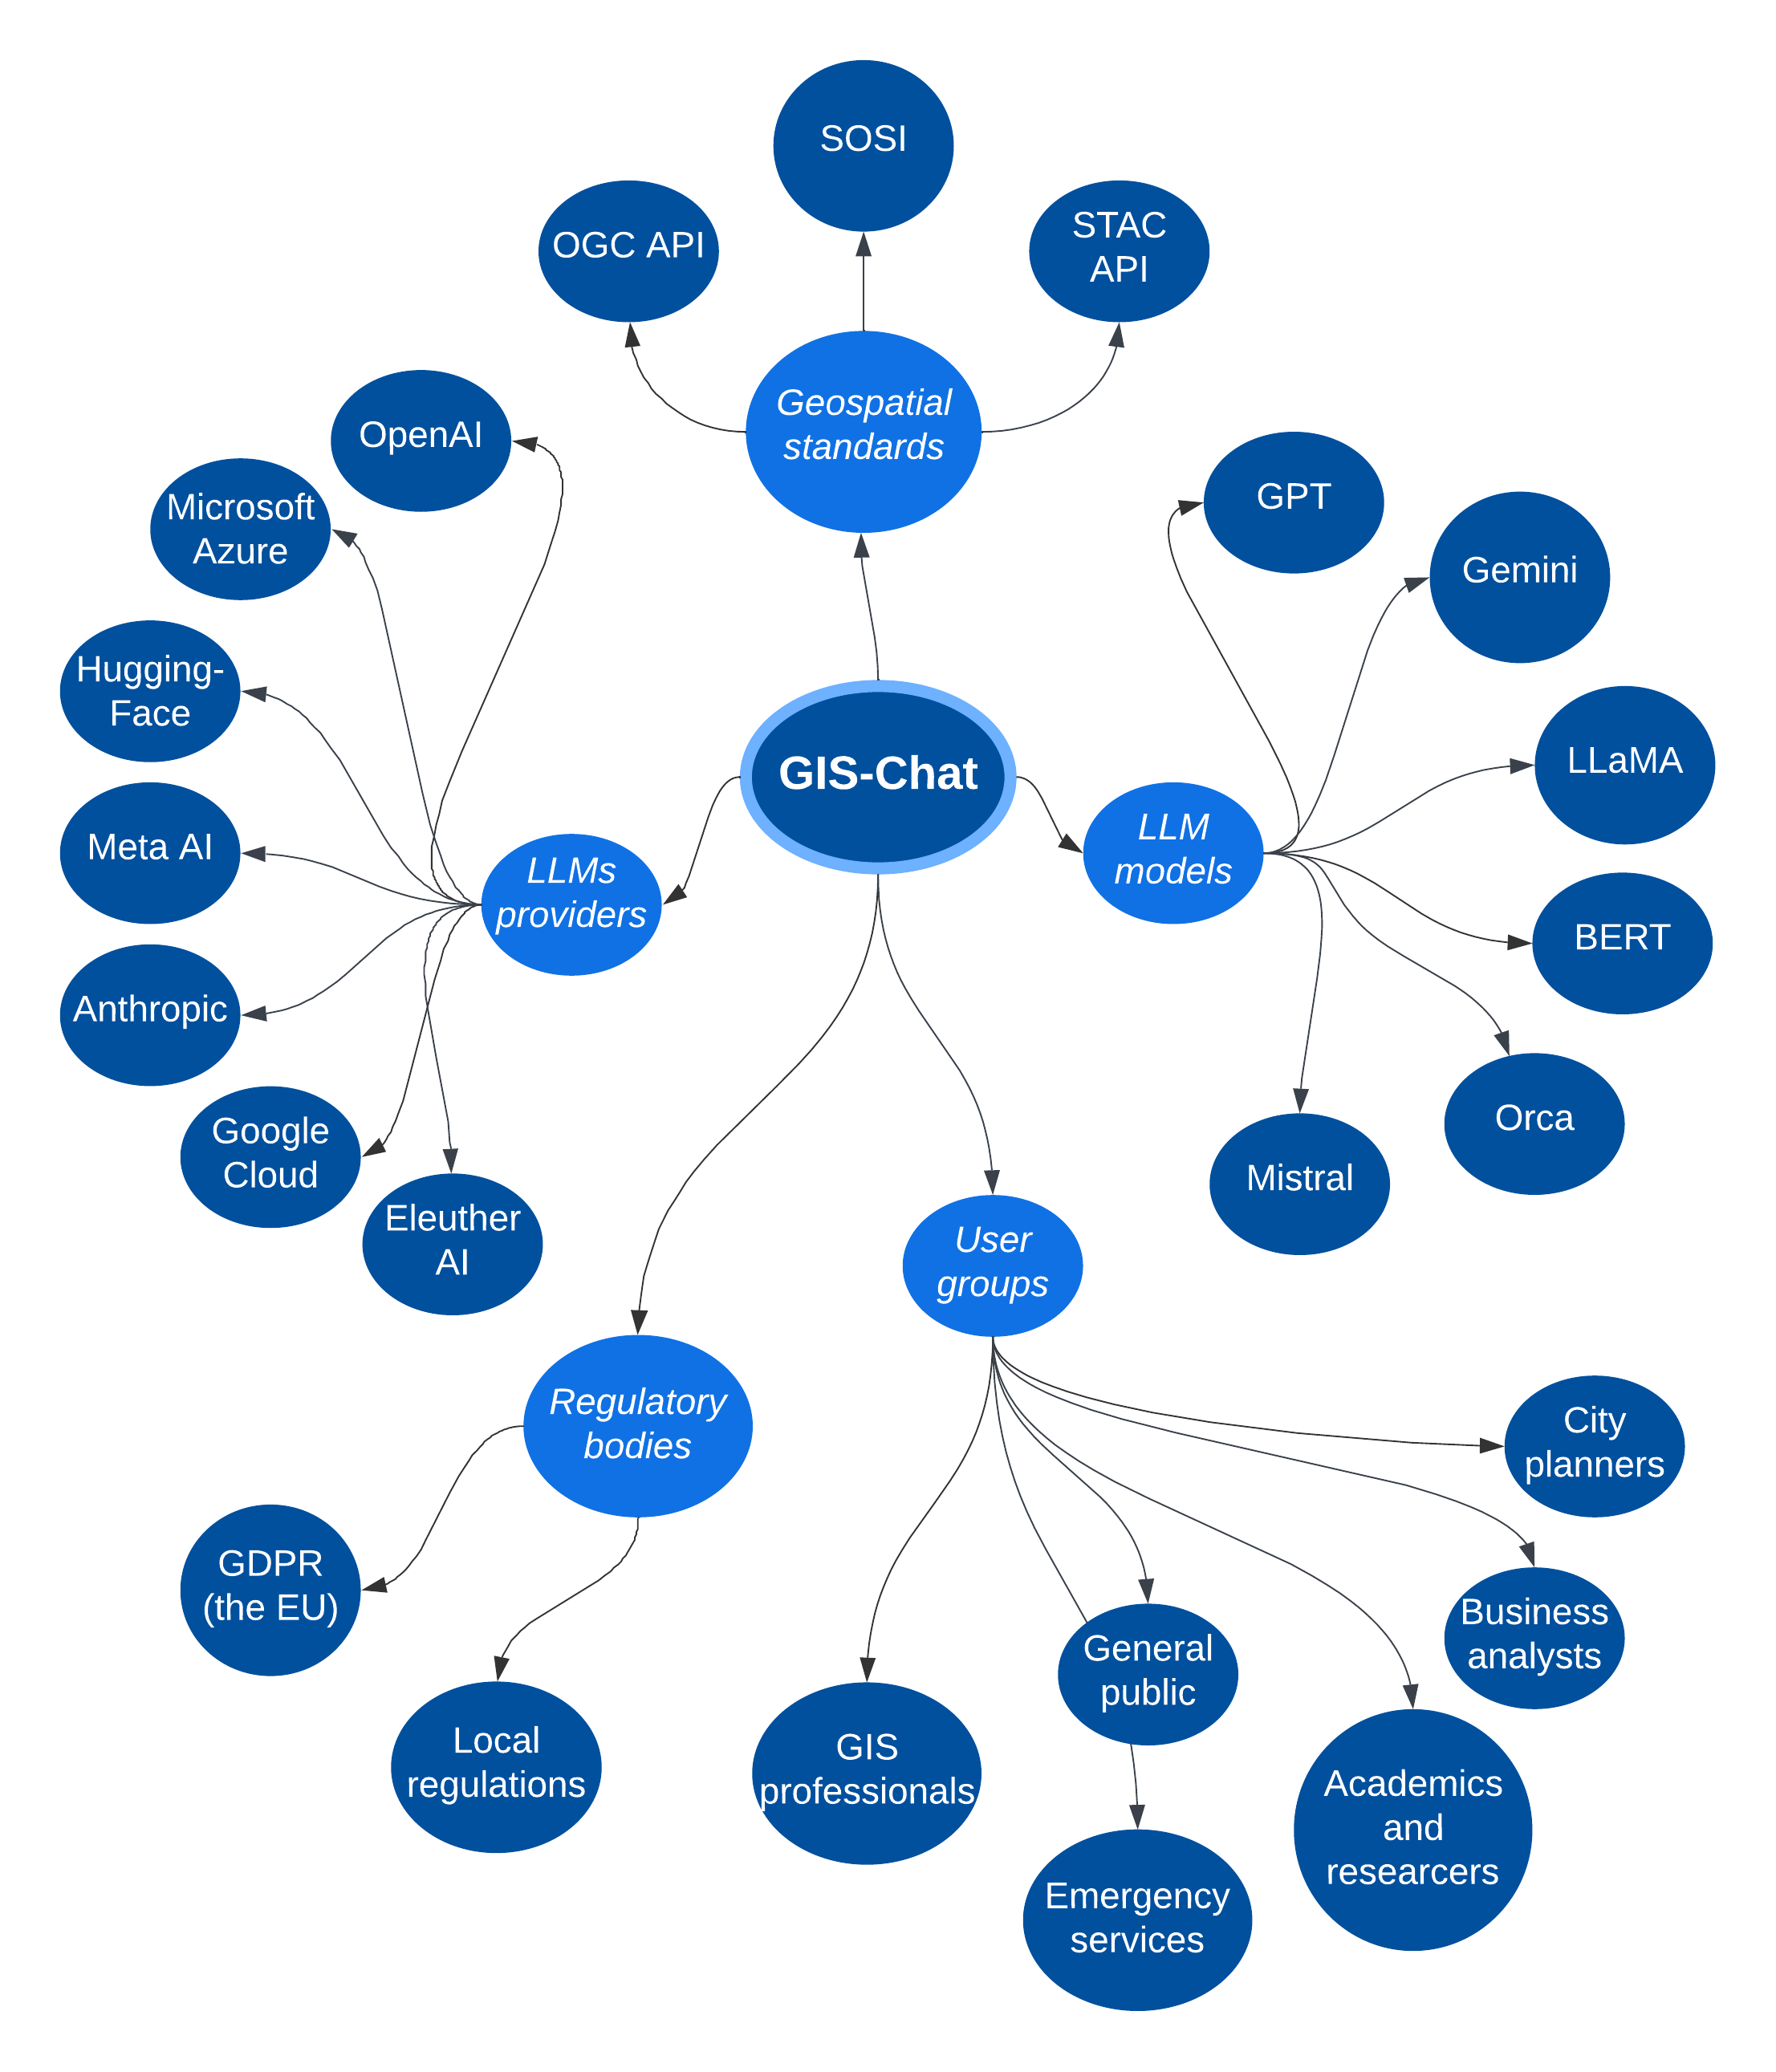
\includegraphics[width=\textwidth]{actor_map}
    \caption{Actor map for stakeholders, providers, and other groups and organizations that could have some relevance to an autonomous LLM-based GIS agent}
    \label{fig:actor-map}
\end{figure}

\section[Large Language Models]{\acrlongpl{acr:llm}}\label{sec:llms}

\glspl{acr:llm} have proved proficient at \gls{acr:nlu} and \gls{acr:nlg}, which are both subfields of \gls{acr:nlp}. \autoref{fig:actor-map} includes six different \acrshortpl{acr:llm} that are all explained in the subsections below. All but the \acrshort{acr:bert} model are made with text generation in mind, with \acrshort{acr:bert} being more adapted for the task of predicting masked tokens, e.g. \enquote{I love going to the \texttt{[MASK]} during summer.}. \acrshort{acr:bert} is very efficient at \gls{acr:nlu}, and is applicable for a wide range of downstream tasks, one of which is discussed in \autoref{subsec:geospatial-context}. As mentioned, the other \acrshortpl{acr:llm} in \autoref{fig:actor-map} are geared towards text generation, with certain members of the \acrshort{acr:gpt} family and Google's Gemini having multimodal capabilities as well. As \autoref{subsec:social-media} will illustrate, these generative models---known for their great conversational abilities and extensive knowledge from pre-training on large corpora---have been found useful in \gls{acr:gis} analysis. The introduction of visual abilities, as seen in newer multimodal models, could potentially even greater enhance such analysis where the visual interpretation of maps is crucial.
% The combination of conversational and visual skills---particularly in multimodal models---holds significant promise for \gls{acr:gis} analysis, where visual interpretation of maps is crucial.

This section will open with an explanation of the fundamental building block of modern \acrlongpl{acr:llm}: the Transformer. \Autosubsectionref{subsec:gpt} and \autoref{subsec:bert} will then discuss the two most famous families of \acrshortpl{acr:llm}, namely the \acrshort{acr:gpt}'s and the \acrshort{acr:bert}'s. \Autosubsectionref{subsec:gemini} will present the brand new multimodal Gemini model from Google, and \autoref{subsec:open-source-llms} will list various open-source alternatives.

\subsection{Attention and The Transformer Architecture}\label{subsec:attention-and-transformers}

\cite{vaswaniAttentionAllYou2017} managed to achieve new state-of-the-art results for machine translation tasks with their introduction of the Transformer architecture. The Transformer has later been proved effective for numerous downstream tasks, and for a variety of modalities. Titling their paper \citetitle{vaswaniAttentionAllYou2017}, \citeauthor{vaswaniAttentionAllYou2017} suggest that their attention-based architecture renders network architectures like \glspl{acr:rnn} redundant, due to its superior parallelization abilities and the shorter path between combinations of position input and output sequences, making it easier to learn long-range dependencies \citep[6]{vaswaniAttentionAllYou2017}.

The Transformer employs self-attention, which enables the model to draw connections between arbitrary parts of a given sequence, bypassing the long-range dependency issue commonly found with \glspl{acr:rnn}. An attention function maps a query and a set of key-value pairs to an output, calculating the compatibility between a query and a corresponding key \citep[3]{vaswaniAttentionAllYou2017}. Looking at \citeauthor{vaswaniAttentionAllYou2017}'s proposed attention function \eqref{eq:attention}, we observe that it takes the dot product between the query $Q$ and the keys $K$, where $Q$ is the token that we want to compare all the keys to. Keys similar to $Q$ will get a higher score, i.e., be \textit{more attended to}. These differences in attention are further emphasized by applying the softmax function. The final matrix multiplication with the values $V$ (the initial embeddings of the input tokens) will yield a new embedding in which all individual tokens have some context from all other tokens. We improve the attention mechanism by multiplying queries, keys, and values with weight matrices that are learned through backpropagation. Self-attention is a special kind of attention in which queries, keys, and values are all the same sequence.

\begin{equation}
    \text{Attention}(Q, K, V) = \text{softmax}\left(\frac{QK^T}{\sqrt{d_k}}\right)V
    \label{eq:attention}
\end{equation}

Attention blocks can be found in three places in the Transformer architecture \citep[5]{vaswaniAttentionAllYou2017} (I will use machine translation from Norwegian to German as an example):

\begin{enumerate}
    \item In the encoder block to perform self-attention on the input sequence (which is in Norwegian)
    \item In the decoder block to perform self-attention on the output sequence (which is in German)
    \item In the decoder block to perform cross-attention (also known as encoder-decoder attention) where each position in the decoder attends to all positions in the encoder
\end{enumerate}

The Transformer represented a breakthrough in the field of \gls{acr:nlp}, and is the fundamental building block of modern \glspl{acr:llm}, most famous of which are the \acrshort{acr:gpt}'s.

\subsection[The GPT Family]{The \acrshort{acr:gpt} Family}\label{subsec:gpt}

\gls{acr:gpt} is a type of \gls{acr:llm} that was introduced by OpenAI in 2018 \citep{radfordImprovingLanguageUnderstanding2018}. Specifically designed for text generation, a \acrshort{acr:gpt} is essentially a stack of Transformer \textit{decoders}. It demonstrates through its vast pre-training on unlabelled data that such unsupervised training can help a language model learn good representations, providing a significant performance boost while alleviating the dependence on supervised learning. While the original Transformer architecture as described by \cite{vaswaniAttentionAllYou2017} was intended for machine translation---thus having encoders to learn the representation of the origin language representation of a given input sequence and decoders to learn the representation in the target language and perform cross-attention between the two---the \acrshort{acr:gpt} is designed only to \textit{imitate} language. This is why there are no encoders to be found in the \acrshort{acr:gpt} architecture, only decoders. The model employs masked multi-head attention (running the input sequence through multiple attention heads in parallel), and is restricted to only see the last $k$ tokens---with $k$ being the size of the context window---and tasked to predict the next one.

Training consists of two stages: unsupervised pre-training and supervised fine-tuning. The former is used to find a good initialization point, essentially teaching the model to imitate the corpora upon which it is trained. This results in a model that will ramble on uncontrollably, just trying to elaborate upon the input sequence it's given to the best of its knowledge. This will naturally produce undefined behaviour, and it is therefore necessary to fine-tune the model on target tasks in a supervised manner. \cite[4]{radfordImprovingLanguageUnderstanding2018} explain how the model can be fine-tuned directly on tasks like text classification, but how one for other tasks needs to convert structured inputs into ordered sequences because the pre-trained model was trained on contiguous sequences of text. In the case of ChatGPT, \citeauthor{openaiIntroducingChatGPT2022} used \gls{acr:rlhf} by employing a three-step strategy: first training using a supervised policy, then using trained reward models to rank alternative completions produced by ChatGPT models, before fine-tuning the model using \gls{acr:ppo}, which is a way of training \acrshort{acr:ai} policies. This pipeline is then performed for several iterations until the model produces the desired behaviour \citep{openaiIntroducingChatGPT2022}.

\subsection[The BERT Family]{The \acrshort{acr:bert} Family}\label{subsec:bert}

\gls{acr:bert}---introduced about four months after \cite{radfordImprovingLanguageUnderstanding2018} presented the \acrshort{acr:gpt} architecture---is a family of language models developed at Google, designed to facilitate a wide range of downstream \gls{acr:nlp} tasks \citep[5]{devlinBERTPretrainingDeep2019}. The \acrshort{acr:bert} architecture consists of stacked bidirectional Transformer \textit{encoders}. This makes \acrshort{acr:bert} unsuitable for text generation, unlike the \textit{decoder}-based \acrshort{acr:gpt} architecture. However, the self-attention mechanism in the encoder---in which tokens can \enquote{see} both past and future tokens---allows for training of deep bidirectional representations. The input sequence is first transformed into embeddings (vector representations). These per-token embeddings include information about the meaning of the word itself, the meaning of the sentence/segment it belongs to, and the token's position in the full input. These embeddings then pass through a stack of Transformer encoders (12 and 24 for \textbf{\acrshort{acr:bert}\textsubscript{BASE}} and \textbf{\acrshort{acr:bert}\textsubscript{LARGE}}, respectively), allowing the model to learn more complex patterns, and patterns of different granularities (token, sentence, document) \citep[5]{devlinBERTPretrainingDeep2019}.

The \acrshort{acr:bert} framework consists of two training steps: pre-training and fine-tuning procedures. \acrshort{acr:bert} is pre-trained on two \gls{acr:nlp} tasks. One of these is \gls{acr:mlm}, in which 15\% of words are masked with the special \texttt{[MASK]} token and are left for the model to predict \citep[4]{devlinBERTPretrainingDeep2019}. The \gls{acr:mlm} task helps the model learn bidirectional representations. The second of these unsupervised tasks is \gls{acr:nsp}, where the special \texttt{[CLS]} token (found at the start of each tokenized sequence) is used to predict if a sentence \texttt{B} follows \texttt{A}. During this pre-training step, the input sequence looks like this:

$$
    \texttt{[CLS]} \text{ this is sentence A } \texttt{[SEP]} \text{ and this is sentence B } \texttt{[SEP]}
$$

\noindent The \texttt{[CLS]} token is used to label sentence B as either \texttt{IsNext} or \texttt{NotNext}.

\acrshort{acr:bert} is normally fine-tuned to specific downstream tasks by utilizing the \texttt{[CLS]} token representation after the last encoder layer, which captures an aggregated representation of the input sequence. This vector representation can then be used as input to a classification layer for tasks like multi-label classification and regression.

\subsection{Gemini}\label{subsec:gemini}

As of writing, Google's Gemini \citep{geminiteamGeminiFamilyHighly2023}---introduced on December 6th 2023---is the latest addition to the ever-growing pool of \acrlongpl{acr:llm}. Being fundamentally designed for multimodality, it is able to reason between text, images, video, audio, and code. It is being released in three different sizes: the Gemini Ultra, the Gemini Pro, and the Gemini Nano. The Gemini Ultra produces state-of-the-art performance on 30 out of 32 widely-used academic benchmarks, and performs worse than \citeauthor{openaiGPT4TechnicalReport2023}'s \acrshort{acr:gpt}-4 on only one benchmark, namely the HellaSwag benchmark for common-sense reasoning for everyday tasks. The Gemini Ultra outperforms \acrshort{acr:gpt}-4 on the \gls{acr:mmlu} benchmark, various reasoning benchmarks, and shows significant improvements in maths- and code-related benchmarks \citep[7]{geminiteamGeminiFamilyHighly2023}. Gemini performs better than \citeauthor{openaiGPT4TechnicalReport2023}'s multimodal equivalent in \acrshort{acr:gpt}-4V on all benchmarks \citep[12]{geminiteamGeminiFamilyHighly2023}. Some of the benchmarks mentioned are discussed further in \autoref{subsec:benchmarks}.

Like the \acrshort{acr:gpt} architecture, Gemini is built on top of Transformer decoders. Gemini is trained to accommodate various modalities, supporting interleaved sequences of text, image, audio, and video as inputs \citep[3-4]{geminiteamGeminiFamilyHighly2023}. This highlights one of the greatest strengths of the Transformer architecture, namely that it can be adapted for multiple modalities. Commonly, multimodal \acrshort{acr:ai} architectures consist of an ensemble of models---one for each given modality---with different representations that can be difficult to combine. The Transformer solves this issue and provides a common architecture that can be trained end-to-end.

\subsection{Open-Source Alternatives}\label{subsec:open-source-llms}

Seeing as the state-of-the-art models of today, like \acrshort{acr:gpt}-4 and Gemini Ultra, are generally closed-source, it is important to note that there are viable open-source alternatives out there. This section lists the most prominent ones.

\subsubsection[LLaMA]{\acrshort{acr:llama}}

Perhaps the most famous family of open-source \acrshortpl{acr:llm} are Meta AI's \acrshort{acr:llama} (\acrlong{acr:llama}) models, with \acrshort{acr:llama} 2 being the latest addition \citep{touvronLlamaOpenFoundation2023a}. \acrshort{acr:llama} 2 is a powerful family of pre-trained and fine-tuned \acrshortpl{acr:llm} that outperformed open-source chat models on most benchmarks at its release. It also shows great results in terms of safety, even outperforming the closed-source ChatGPT-0301 model. The training process of \acrshortpl{acr:llama} is similar to that of the \acrshort{acr:gpt} model, with pre-training being performed using an optimized autoregressive transformer which is trained from a large corpus of unstructured data. \acrshort{acr:llama} is then fine-tuned using various alignment techniques, and the authors also share a new technique called Ghost Attention, which aims to control dialogue flow over multiple turns. \gls{acr:rlhf} and \gls{acr:ppo} are other important techniques used to get the desired behaviour out of the model.

Many flavours of \acrshort{acr:llama} have been trained. Most notably is Code \acrshort{acr:llama} 2 \citep{roziereCodeLlamaOpen2023}, a family of \acrshortpl{acr:llm} fine-tuned for code, scoring at 53\% and 55\% on the HumanEval and \gls{acr:mbpp} benchmarks, respectively. Vicuna-13B is another example of a \acrshort{acr:llama}-based model, and is fine-tuned on user-shared conversations collected from ShareGPT\footnote{\url{https://sharegpt.com/}}, a website where users can upload ChatGPT conversations. At its release in March 2023, it achieved more than 90\% quality of OpenAI's ChatGPT and Google's Bard, while also outperforming the original \acrshort{acr:llama} model.

\subsubsection{Mistral}

Mistral 7B \citep{mistralaiMistral7B2023} is another open-source \acrshort{acr:llm}, and is claimed by its creators at Mistral \acrshort{acr:ai} to be \enquote{the most powerful language model for its size to date}. Being a 7.3B parameter model, it is quite small compared to other models, such as the 1.76T parameter \acrshort{acr:gpt}-4 model. Mistral 7B outperforms the \acrshort{acr:llama} 2 13B on all benchmarks, and approaches Code \acrshort{acr:llama} 7B performance on code.

\subsubsection{Orca 2}

Orca 2 \citep{mitraOrcaTeachingSmall2023}---developed at Microsoft---is an open-source \acrshort{acr:llm} with exceptional step-by-step reasoning capabilities. It is based on \acrshort{acr:llama} 2 and is fine-tuned on curated training data from a more capable teacher model, like \acrshort{acr:gpt}-4. Evaluation results show that the Orca-2-13B model surpasses models of the same size, and that it is competitive with models 5-10x larger, exceeding the performance of \acrshort{acr:llama}-2-Chat70B and performing comparably to ChatGPT on reasoning tasks \citep[11-12]{mitraOrcaTeachingSmall2023}. It does have some limitations, most notably in terms of potential of misuse due to the lack of suitable safeguards like \gls{acr:rlhf} training \citep[21]{mitraOrcaTeachingSmall2023}.



\section[Large Language Model Providers]{\acrlong{acr:llm} Providers}\label{sec:llm-providers}

The \acrshort{acr:ai} community called Hugging Face\footnote{\url{https://huggingface.co/}} is the most widely used hub for open-source and open-science machine learning. It is used by both individual community members and large commercial actors like Google Cloud and Meta \acrshort{acr:ai} as a way of contributing to the world open-source \acrshort{acr:ai}. Hugging Face's \texttt{transformers}\footnote{\url{https://github.com/huggingface/transformers}} Python library provides an interface with their hub, which at the time of writing has 177k stars on GitHub.

OpenAI is one of the leading providers of \acrshortpl{acr:llm}, most prominently through their \acrshort{acr:gpt} series. While originally founded as an open-source company, their models are now closed-source and their \acrshort{acr:gpt} \acrshortpl{acr:api} are paid services. It should be noted, however, that they still are great contributors to open-source \acrshort{acr:ai}, having uploaded a range of speech detection and diffusion models to Hugging Face.

Microsoft Azure---the main partner of OpenAI---provides \acrshortpl{acr:api} for OpenAI's language models, including the \acrshort{acr:gpt}-4, \acrshort{acr:gpt}-3.5-Turbo, and Embeddings model series. Unlike OpenAI's own \acrshortpl{acr:api}, Microsoft Azure offers private networking, regional availability, and responsible \acrshort{acr:ai} content filtering.\footnote{\url{https://learn.microsoft.com/en-us/azure/ai-services/openai/overview?source=recommendations}} Also, by using Microsoft Azure's \acrshort{acr:api}, \acrshort{acr:llm} inputs and outputs are unavailable to OpenAI, which is not the case otherwise.\footnote{\url{https://learn.microsoft.com/en-us/legal/cognitive-services/openai/data-privacy}}

\cite{clearyLatencyBenchmarksComparisons2023} did benchmarking of different \acrshortpl{acr:llm} on different providers. Important takeaways were that \acrshort{acr:gpt}-4 is about 6.3 times slower than \acrshort{acr:gpt}-3.5-Instruct, and that Microsoft Azure has far lower latency in most cases for inference on \acrshort{acr:gpt} models, compared to OpenAI's own \acrshortpl{acr:api}. Such considerations are important when addressing usability of \acrshort{acr:llm}-based applications, balancing accuracy against speed and cost.

Aforementioned Google Cloud is another important \acrshort{acr:llm} provider. They provide a wide range of services, among these the Vertex \acrshort{acr:ai} platform.\footnote{\url{https://cloud.google.com/vertex-ai/}} Vertex \acrshort{acr:ai} provides \acrshort{acr:api} access to foundational models through the Model Garden platform which supports first-party, open-source, and third-party models. Vertex \acrshort{acr:ai} also provides experimental prompt design and fine-tuning services, and \acrshort{acr:ai} is a paid service.

Anthropic\footnote{\url{https://www.anthropic.com/}} is another closed-source \acrshort{acr:llm} provider, and has grown rapidly in size since their launch in 2021. They focus on creating safer, steerable, and more reliable models. Their flagship model is Claude 2.1, which has a large context window of 200,000 tokens, enabling users to upload large technical documentation that the model can keep in its memory when generating responses. Anthropic lists complex reasoning, creativity, and coding as Claude's major strengths.

There are numerous open-source alternatives to these closed-source resources. Using free open-source alternatives where possible is a good option to reduce cost. Meta \acrshort{acr:ai}\footnote{\url{https://ai.meta.com/}} is a big contributor to open-source \acrshort{acr:ai}, most famously through Pytorch---a popular deep learning framework---and their LLaMA models (see \autoref{subsec:open-source-llms}). Eleuther \acrshort{acr:ai}\footnote{\url{https://www.eleuther.ai/}} is an open-source-centred company with the aim to \enquote{increase transparency and reduce potential harms from emerging \acrshort{acr:ai} technologies}. As such, they have released a range of trained \acrshortpl{acr:llm} along with the codebases used to train them. Perhaps most famous is their \acrshort{acr:gpt}-J model, which is an autoregressive model in the style of \acrshort{acr:gpt}-3, aimed at the English language.

\section{Geospatial Standards}\label{sec:geospatial-standards}

It is important for \acrshort{acr:gis} applications of any kind to support modern geospatial standards. \Autosubsectionref{subsec:standardization-international} will offer a brief overview of the standardization efforts on the international stage, while \autoref{subsec:standardization-norway} will similarly cover these efforts within the context of Norway.

\subsection{International Standardization Work}\label{subsec:standardization-international}

International geospatial standardization involves the global collaboration and development of uniform standards and protocols for geospatial data and technologies. The \acrshort{acr:ogc} standards and the \acrshort{acr:stac} \acrshort{acr:api} standard are examples of such work.

\subsubsection[OGC Standards]{\acrshort{acr:ogc} Api Standard}\label{subsubsec:ogc}

The \gls{acr:ogc} \acrshort{acr:api} standards serve as the glue in the field of \gls{acr:gis}, paving the way for interoperability and data exchange between diverse systems. Supporting multiple data formats including \acrshort{acr:json}, \acrshort{acr:gml}, and \acrshort{acr:html}, the \gls{acr:ogc} \acrshort{acr:api} standard provides a modular architecture consisting of a core specification and various extensions. According to their webpages, they provide 80 different standards, each for a specific geospatial purpose. Notable examples are 3D Tiles, CityGML, GeoTiff, and \acrshort{acr:ogc} \acrshort{acr:api} - Features \citep{ogcOGCStandards2023}. The \acrshort{acr:ogc} \acrshort{acr:api} standards function as modern replacements to older standards like \acrshort{acr:wms} and \acrshort{acr:wfs}, and presents a more adaptable framework for spatial data operations, facilitating innovation in the \acrshort{acr:gis} domain.

\subsubsection[The STAC Api Standard]{The \acrshort{acr:stac} Api Standard}\label{subsubsec:stac}

The \gls{acr:stac} \acrshort{acr:api} is a standardized way to expose collections of spatio-temporal data for online search and discovery. Built upon a \acrshort{acr:json} core, it aims to be a uniform and flexible environment from which developers can customize the API infrastructure to their domain. \acrshort{acr:stac} is closely related to \acrshort{acr:ogc}, and \acrshort{acr:ogc} board member Chris Holmes said the following in a blog post: \enquote{The \acrshort{acr:stac} \acrshort{acr:api} implements and extends the \gls{acr:ogc} \acrshort{acr:api} - Features standard, and our shared goal is for \gls{acr:stac} \acrshort{acr:api} to become a full \gls{acr:ogc} standard.} \citep{holmesSpatioTemporalAssetCatalogs2021}. \gls{acr:stac} \acrshort{acr:api} provides a powerful query language that allows users to search by various parameters like time, location, and keywords, making it widely applicable. The \acrshort{acr:stac} community has also defined specifications in order remove the complexity associated with having to create unique pipelines when consuming different spatio-temporal collections. The significance of the \gls{acr:stac} \acrshort{acr:api} lies in its ability to democratize access to large volumes of geospatial data. By offering a common standard for data cataloguing and discovery, it reduces the barriers that often exist due to incompatible data formats. Developers or \acrshort{acr:gis} professionals can take advantage of this through built-in tooling in QGIS---a desktop \gls{acr:gis} for viewing, editing, and analysing spatial data---or through third-party packages in the Python and R programming languages. The API is also accessible through the command line interface when using \acrshort{acr:gdal} \citep{STACTutorials}.

\subsection{Norwegian Standardization Work}\label{subsec:standardization-norway}

Geospatial standardization work has been on the agenda of Norwegian governing powers for decades and have materialized in frameworks/collaborations like \nameref{subsubsec:geovekst} and \nameref{subsubsec:norge-digitalt}, as wells as the \nameref{subsubsec:sosi} file format. This standardization work will be the topic of \autoref{subsec:standardization-norway}.

\subsubsection[SOSI]{\acrshort{acr:sosi}}\label{subsubsec:sosi}

\gls{acr:sosi} is a Norwegian file format for storing and exchanging geospatial data. It was first introduced in 1987 and has since approached international standards, with the most important arenas being \acrshort{acr:iso}/\acrshort{acr:tc} 211 and \gls{acr:ogc} \citep{mardalNasjonalStrategiVidereutvikling2015}. \gls{acr:sosi} is the adopted Norwegian standard for creating and delivering digital geographic data. It is administered by the Norwegian Mapping Authority \citep{maehlumSOSI2023}.


In a \gls{acr:sosi} dataset, terrain points, lines, and polygons are represented by their coordinates and classified into various object types according to the \gls{acr:sosi} object catalogue standard. However, there are few GIS systems that can read \gls{acr:sosi} data directly, so data in \gls{acr:sosi} format usually needs to be converted into more \gls{acr:gis}-friendly data formats \citep{maehlumSOSI2023}.

\subsubsection{Geovekst}\label{subsubsec:geovekst}

Geovekst is a Norwegian initiative that aims for collaborative collection, distribution, management, and maintenance of geospatial information. It was established in 1992, and is a partnership between national, regional, and local government bodies, as well as several private companies.\footnote{\url{https://www.kartverket.no/geodataarbeid/geovekst}} The primary goal associated with Geovekst is to \enquote{collaborate to secure updated Geovekst data to help solve parts of the parties' societal missions} \citep[5]{thenorwegianmappingauthorityHandbokGeovekstsamarbeidet2023}. The objective of the collaboration is to ensure that geographical data is collected \textit{once}, conforming  to \textit{one} standard, maintained in \textit{one} place, and used by \textit{many}. Responsibilities and costs are shared among the parties of the collaboration.

The most important contribution of Geovekst is \gls{acr:fkb}, a series of very detailed Norwegian mapping datasets, serving as rich resources for both public and private sectors. The datasets are obtained through a variety of data sources, including aerial photographs, laser scans, and manual mapping. Geovekst also provides airborne surveys in emergency situations, when the speed of surveying is important.\footnote{\url{https://www.kartverket.no/geodataarbeid/geovekst/datafangst-i-krise}}

\subsubsection[The National Spatial Data Infrastructure]{The \acrlong{acr:nsdi}}\label{subsubsec:norge-digitalt}

Established in 2005, the \gls{acr:nsdi} is a more recent framework compared to Geovekst, and is more often referred to by its Norwegian name: \textit{Norge Digitalt}. The \gls{acr:nsdi} involves governmental bodies (national, regional, and municipal), but also educational and research institutions and companies with responsibilities on a nation-wide scale, examples of which include Telenor and local and regional energy companies \citep[6]{norgedigitaltGenerelleVilkarNorge2023}. The \gls{acr:nsdi} infrastructure is the sum of common standards and rules, geographical data and services related to these, in addition to tools and deals. It aims to coordinate geospatial activities in Norway, making it easier to discover, access, and use spatial data. The framework is coordinated by the Norwegian Mapping Authority \citep{norgedigitaltGenerelleVilkarNorge2023}.



\section{User Groups}\label{sec:user-groups}

\begin{table}[ht]
    \centering
    \begin{tabular}{l|c}
        \toprule
        \textbf{Category}                    & \textbf{Percentage} \\
        \midrule
        Task oriented                        & 23.1\%              \\
        Informational                        & 20.2\%              \\
        Social                               & 16.2\%              \\
        Personal advice and self-improvement & 13.1\%              \\
        \bottomrule
    \end{tabular}
    \caption{Distribution of query categories \citep{kumarWhatArePeople2023a}}
    \label{tbl:query-category-distribution}
\end{table}

There are several user groups that could take advantage of an \acrshort{acr:llm}-based agent with extensive geographic and \acrshort{acr:gis}-related knowledge. Queries to such an agent could span from simple retrieval questions like \enquote{How many people live in Trondheim?} and \enquote{What is Sweden's third largest city?}, to more complicated questions that require problem-solving abilities and reasoning. While it is difficult to obtain good datasets of common queries, \cite{kumarWhatArePeople2023a}---creator of the chatbot app \textit{Pocket AI}\footnote{\url{https://github.com/varunon9/pocket-ai}}---shared a dataset of \textasciitilde 13k user queries from his app along with classifications of these. Salient categories are listed in \autoref{tbl:query-category-distribution}. The main takeaway from these numbers is that the main motivation for use is productivity.

\begin{table}[ht]
    \centering
    \begin{tabular}[t]{l|c}
        \toprule
        \textbf{Category}              & \% \textbf{(n)} \\
        \midrule
        Productivity                   & 55\% (109)      \\
        Novelty                        & 51\% (101)      \\
        Fun and amusement              & 20\% (41)       \\
        Creative work                  & 18\% (34)       \\
        Social interaction and support & 9\% (18)        \\
        Other                          & 7\% (15)        \\
        \bottomrule
    \end{tabular}
    \caption{Categories and frequency of ChatGPT usage \citep[16-17]{skjuveWhyPeopleUse2023}}
    \label{tbl:chatgpt-motivation-survey-restuls}
\end{table}

This aligns with the results of \cite{skjuveWhyPeopleUse2023} from their questionnaire-based study performed in late January 2023, about two months after the release of ChatGPT. The goal of their study was to figure out why people use ChatGPT. They found that most participants (55\%) are motivated by productivity, specifically applying it for routine tasks, information retrieval, text generation and writing support, and software development \citep[17-21]{skjuveWhyPeopleUse2023}. \autoref{tbl:chatgpt-motivation-survey-restuls} shows all categories and their frequencies. There were 197 samples in total, and more than one category could be  assigned to each sample. It is worth noting that the study is likely to have included early adopters, which could make the results less representative for the time at which this report is written (\today), now that use patterns have become more established \citep[37]{skjuveWhyPeopleUse2023}.

The main reason why people use conversational \acrshort{acr:ai} is clearly to increase their productivity, whether in a professional, academic, or personal context. 67 out of the 197 participants in \citeauthor{skjuveWhyPeopleUse2023}'s study highlighted ChatGPT's ability to understand complex queries and that it is \enquote{efficient in alleviating the need to experiment with different phrasings of the query} \citep[18]{skjuveWhyPeopleUse2023}, as is often needed when 'Googling' for an answer to a specific question. The ease of information retrieval, along with it's problem-solving abilities \citep[20]{skjuveWhyPeopleUse2023}, could also make conversational \acrshortpl{acr:ai} highly relevant for \acrshort{acr:gis}-related purposes.

One could imagine a range of potential user groups that could benefit from such an artificial, and spatially aware, companion. Some suggested user groups are presented in \autoref{fig:actor-map}. Perhaps the most obvious one is that of the \acrshort{acr:gis} professionals. While an \acrshort{acr:ai}-based \acrshort{acr:gis} agent more capable than the average \acrshort{acr:gis} professional is currently far from becoming a reality, such an agent could help suggest strategies of solving a particular problem using the input data available and a good user prompt, or it could help solve mundane tasks in an automated way in order to allow \acrshort{acr:gis} professionals to allocate more time to creative and complex tasks.

Closely related to \acrshort{acr:gis} professionals are the city planners. Though often less knowledgeable in the field of \acrshort{acr:gis}, they are increasingly dependent upon geospatial analyses in order to make informed decisions. Having an easy-to-use \acrshort{acr:gis} agent ready at any moment could prove both time- and cost-saving. The same goes for business analysts and people involved in academia. The \textit{time} variable is especially important to the emergency services. At the impact of a natural disaster like a flood or forest fire, geospatial analysis could prove lifesaving. Having powerful geospatial knowledge even in the absence of a \acrshort{acr:gis} professional is therefore important in order to focus resources to areas where the situation is most pressing.

An \acrshort{acr:llm}-based agent with geospatial awareness could also be useful to the general public: one may want to find suitable biking routes or good hills for interval running, or to identify areas prone to flooding when buying a house. Most people do not possess the knowledge or time to perform such analyses themselves, so an automated \acrshort{acr:ai}-based agent could prove useful for such use cases.



\section{Ethical and Privacy Concerns}\label{sec:ethical-and-privacy-concerns}

Although an \acrshort{acr:llm}-based \acrshort{acr:gis} agent could prove powerful, there are some ethical pitfalls in terms of regulations and privacy concerns that need consideration. If such an agent is to make decision on behalf of humans it is important that one can hold someone accountable in the case that something goes wrong. If an \acrshort{acr:ai}-based agent is tasked to lead firefighters to the tactically optimal locations in order to quench a fire, but  instead misleads them and traps them inside the fire, who is then to blame? \cite{sparrowKillerRobots2007} provides an interesting angle on such issues, though in his essay related the role of artificially intelligent robots in modern warfare.

Furthermore, it is vital to ensure that \acrshort{acr:ai} agents are not utilized for immoral purposes, like finding the optimal location in which to dissolve poison into people's drinking water to maximize the number of people killed. Work has been done with newer \acrshortpl{acr:llm} to prevent them from producing dangerous, misinformed, or toxic text---this issue is widely discussed in the technical report of the \acrshort{acr:gpt}-4 model \citep[11-14]{openaiGPT4TechnicalReport2023}---but there have been cases where these issues haven't been considered well enough.\footnote{The \acrshort{acr:llama}-based Alpaca model, developed at Stanford University, was taken offline after being shown to produce misinformation, toxic text: \url{https://www.theregister.com/2023/03/21/stanford_ai_alpaca_taken_offline/}}

The \gls{acr:gdpr} entered into applicability in the European Union on 25th of May 2018, and although not a member of the European Union, Norway incorporated the \gls{acr:gdpr} in July the same year due to its membership of the European Economic Area. The \gls{acr:gdpr} imposes stricter regulations about data privacy, meaning people have more control over their personal data, and that businesses get a level playing field in terms of what customer information is available \citep{datatilsynetGeneralDataProtection}. With data privacy arguably being more relevant than ever, we must make certain that \acrshort{acr:llm}-based \acrshort{acr:gis} agents are unable to access and spread information of private or sensitive character, even if such information has become publicly available by accident---as was the case when the Norwegian Broadcasting Corporation (NRK) was able to (legally) obtain accurate geolocations of central people in the Norwegian army from a commercial London-based company\footnote{Link to news article in Norwegian: \url{https://www.nrk.no/norge/xl/norske-offiserer-og-soldater-avslort-av-mobilen-1.14890424}}.

\glsresetall
\chapter{Related Work}
\label{cha:related_work}

\begin{comment}
What other research has been conducted in this area and how is it related to your work?
This section is thus where your literature review will be presented. It is important when presenting the review
that you give an overview of the motivating elements of the work going on in your field and how these relate to your work,
rather than a list of contributors and what they have done.
This means that you need to extract the key important factors for your work and discuss how others have addressed
each of these factors and what the advantages/disadvantages are with such approaches.
As you mention other authors, you should reference their work.
Note that the reference list reflects the literature you have read {\em and\/} have cited.
This will only be a subset of the literature that you have read.

A good way to find relevant work is by checking what others are referencing, e.g., in papers you have already found
or in previous studies carried out at NTNU, such as \cite{Berg;Gopinathan:17}.
However, when doing that,
do not fall into one of the common traps, such as re-iterating someone's false quote or faulty analysis of
a previous paper (check the original source!), or getting stuck inside a local research cluster (a group of
researchers that mainly refer to the ones using the same type of approaches or similar ideas).

Make sure that it is clear how and why you decided to include some references (and discard others). As in all parts of research, it should ideally be possible for someone else to reproduce your work, also when it comes to finding the relevant references.
There are (at least) three basic methods for finding references:
\begin{enumerate}
    \item Trust the authorities (e.g., your supervisor) to dig out good texts for you.
          Those can often be used as a seed set for:
    \item Snowballing, where you have some good articles and check the references in them for other good ones.
          Note that this can be done both backwards and forwards on the timeline; that is, using tools like Google Scholar, you can also check who refers \textit{to\/} the good articles you have already found.
    \item Carry out a Systematic Literature Review (or Structured Literature Review, SLR), a method introduced more formally into Software Engineering by \citet{Kitchenham;Charters:07}, but based on several similar methods for other disciplines.
          At the core of the method is an SQL-related  search over a reference database (such as Google Scholar).
          A good introduction to SLR is given by \citet{Kofod-Petersen:14}.
\end{enumerate}

Note that a reference needs to be complete: you should always give the full name of a conference or journal,
always include page numbers, always say where a book or thesis was published, and where a conference took place, as further described in Section~\ref{sec:reference_list}.

Just as described in the Background chapter (Chapter~\ref{cha:background_theory}), it is possible (and even likely) that you will want to reuse some of the text that you have written for your specialisation project in your Master's Thesis.
This is allowed, as long as it is clearly stated what you have reused and in what form (e.g., if a section is a straight-forward copy, if it has undergone only editorial changes, if it contains some old material but also some new, etc.).
\end{comment}

\glsresetall
\chapter{Experiments}
\label{cha:experiments}

\Autosectionref{sec:experimental-setup} of the \nameref{cha:experiments} chapter will describe the methodology and rationale behind the two experiments conducted in this thesis. The first experiment, presented in \autoref{subsec:benchmarking-setup}, assesses GeoGPT's ability to solve common \acrshort{acr:gis} tasks through a new \acrshort{acr:gis} benchmarking dataset. The other experiment, presented in \autoref{subsec:prompt-quality-test-setup}, will assess the importance of the quality of the prompt passed from the user to GeoGPT. \Autosectionref{sec:datasets} lists the datasets used in the experiments. \Autosectionref{sec:experimental-results} presents the experimental results and offers interpretations of the findings from the experiments. It will also present several example results, including screenshots of the application and code that generated by GeoGPT.

\section{Experimental Setup}
\label{sec:experimental-setup}

\begin{comment}
Trying and failing is a major part of research. However, to have a chance of success you need a plan driving the experimental research, just as you need a plan for your literature search. Further, plans are made to be revised and this revision ensures that any further decisions made are in line with the work already completed.

The plan should include what experiments or series of experiments are planned and what questions the individual or set of experiments aim to answer. Such questions should be connected to your research questions, so that in the evaluation of your results you can discuss the results wrt to the research questions.
\end{comment}

\begin{comment}
The experimental setup should include all data --- parameters, etc. --- that would allow a person to repeat your experiments.
This will thus be the actual instantiation for each experiment of the general architecture described in Chapter~\ref{cha:architecture}.
\end{comment}

% The experiments conducted using the above-mentioned \acrshort{acr:gis} benchmark are divided into two approaches. The first approach, presented in \autoref{subsec:benchmarking-setup}, is intended to evaluate GeoGPT's ability to solve a variety of geospatial tasks. The second approach, presented in \autoref{subsec:prompt-quality-test-setup}, aims to uncover the importance of the quality of the initial user prompt. \Autosubsectionref{subsec:hardware-and-model-version} describes the hardware on which the experiments were executed, and the specific \acrshortpl{acr:llm} that were used.

This section will explain the concept and setup of the two experiments mentioned in the paragraph above. \Autosectionref{subsec:benchmarking-setup} will describe the setup for the \acrshort{acr:gis} benchmark experiments, while \autoref{subsec:prompt-quality-test-setup} will explain the setup for the prompt quality experiment. \Autosubsectionref{subsec:hardware-and-model-version} describes the hardware on which the experiments were conducted, and the specific \acrshortpl{acr:llm} that were used.

\subsection[GIS Benchmark Experiment]{\acrshort{acr:gis} Benchmark Experiment}
\label{subsec:benchmarking-setup}

% In order to investigate how an \acrshort{acr:llm}-based \acrshort{acr:gis} agent most comfortably accesses geospatial data, a decision was made to include three different methods for data access in the experiments. The first method for data access is to have the files described in \autoref{sec:datasets} remain untouched. The files would be stored locally on the computer on which the experiments are conducted, and GeoGPT, which runs on the same computer, would be able to interact with the data through the code it generates. These files are made available in GeoGPT's working directory. The second method used is to load the data into a spatial \acrshort{acr:sql} database and provide the model with database schemas that can be used to generate queries. The datasets were uploaded to a Dockerized PostGIS database using QGIS's DB Manager plugin. The third method for data access is to use the \acrshort{acr:ogc} \acrshort{acr:api} Features standard. This method exposes the data stored in the PostGIS database through a web \acrshort{acr:api} that allows consumers of the \acrshort{acr:api} to download the data over \acrshort{acr:http} as GeoJSON.

The first experiment will measure the abilities of GeoGPT three agent types to produce correct answers. It will also measure cost and time taken to generate answers, and the agent's ability to produce similar answers consistently (repeatability). To do this, a benchmarking dataset was constructed. This is a set of 12 GIS-related questions with corresponding correct answers, and can be viewed in its entirety in \autoref{tbl:questions-quantitative}. The \acrshort{acr:gis} benchmark experiment will seek to compare the performance of GeoGPT's three agents. Each of the 12 questions will be asked three times per agent type. Thus, the total number of test runs becomes the following:

$$12 \text{ questions} \cdot 3 \text{ agent types} \cdot 3 \text{ repetitions} = 108 \text{ tests}$$

The following sections, named \enquote{\nameref{subsubsec:outcome-evaluation}}, \enquote{\nameref{subsubsec:cost-and-duration}}, \enquote{\nameref{subsubsec:repeatability}}, will go into detail on the different ways that the results are evaluated.

\subsubsection{Outcome Evaluation}
\label{subsubsec:outcome-evaluation}

Each of the 108 GeoGPT-generated answers will be manually evaluated based on how well the question was answered, and this outcome will be annotated as one of the following: \textit{success}, \textit{partial success}, and \textit{failure}. \autoref{tbl:test-outcome-enum} shows the guidelines used when assigning outcome scores.

\begin{table}[htbp]
    \centering
    \caption[Guidelines for evaluating outcome of tests]{Guidelines for evaluating outcome of tests}
    \label{tbl:test-outcome-enum}
    \begin{tabularx}{0.9\textwidth}{p{3cm}X}
        \toprule
        \textbf{Outcome} & \textbf{Guideline}                                                                                                                                                                                  \\
        \midrule
        Success          & The question was answered correctly and little to no follow-up from the user was required to produce the desired outcome. No false assumptions were made by the system when answering the question. \\
        Partial Success  & Portions of the question were answered correctly or semi-correctly, and/or some follow-up from the user was required to guide the system toward the solution.                                       \\
        Failure          & The question was answered incorrectly, and/or false assumptions were made by the system while attempting to answer the question.                                                                    \\
        \bottomrule
    \end{tabularx}
\end{table}


\subsubsection{Cost and Duration}
\label{subsubsec:cost-and-duration}

The application is hooked up to LangChain AI's tracing system, \textit{LangSmith}.\footnote{\url{https://www.langchain.com/langsmith} (last visited on 2nd June 2024)} Apart from being a useful tool for debugging purposes, it provides a simple way to obtain detailed data on token and time usage for a particular run, as well as the total cost of the run, in American dollars. Further details, and screenshots of LangSmith's interface, can be found in \autoref{app:langsmith}.

Box plots will be used to compare these three metrics for the different agents. The box plots follow the description for box plots found on Wikipedia.\footnote{\url{https://matplotlib.org/stable/api/_as_gen/matplotlib.pyplot.boxplot.html} (last visited on 2nd June 2024)}\footnote{\url{https://en.wikipedia.org/wiki/Box_plot} (last visited on 2nd June 2024)} Box plots allow us to easily see where the 0th ($Q_0$), 25th ($Q_1$), 50th ($Q_2$), 75th ($Q_3$), and 100th ($Q_4$) percentiles of the datasets lie, as well as the dataset's outliers. Outliers are those data points that fall more than 50\% outside the interquartile range, which is the distance between $Q_3$ and $Q_1$ in each direction.

\subsubsection{Repeatability}
\label{subsubsec:repeatability}

Another aspect that the \acrshort{acr:gis} benchmark experiment will try to evaluate, is the consistency of the system --- its ability to produce similar responses, repeatedly. The outcomes scores are encoded using the ordinal encoding presented \autoref{tbl:outcome-encoding}. A higher value indicates a better outcome. Standard deviations are calculated for each triplet of identical test samples (samples where the question and the agent type remained the same), using these encoded outcomes. This will serve as a suitable measure for assessing repeatability.

\begin{table}[htbp]
    \centering
    \caption{Ordinal encodings for outcome scores}
    \label{tbl:outcome-encoding}
    \begin{tabularx}{0.5\textwidth}{XX}
        \toprule
        \textbf{Outcome} & \textbf{Encoded Value} \\
        \midrule
        Success          & 2                      \\
        Partial Success  & 1                      \\
        Failure          & 0                      \\
        \bottomrule
    \end{tabularx}
\end{table}


\subsection{Prompt Quality Experiment}
\label{subsec:prompt-quality-test-setup}

A second experiment is constructed to evaluate the importance of the initial question/prompt from the user. As stated in the \nameref{sec:background-and-motivation} chapter, part of the motivation for developing an \acrshort{acr:llm}-based \acrshort{acr:gis} like GeoGPT is to make \acrshort{acr:gis} more accessible to non-experts. It is therefore interesting to assess the extent to which a carefully constructed prompt by a \acrshort{acr:gis} expert can enhance the system's output.

For these experiments, the three hardest questions from the \acrshort{acr:gis} benchmark experiment were picked. Then, for each of these three questions, a \textit{novice}-level and an \textit{expert}-level prompt was constructed. The novice-level prompt is as simple as possible, while the expert-level prompt is more elaborate and written as a step-by-step recipe for solving the problem. Despite their differences, the prompts should ideally produce the same answer.

\subsection[Hardware and LLM Version]{Hardware and \acrshort{acr:llm} Version}
\label{subsec:hardware-and-model-version}

All experiments were conducted on a Lenovo ThinkPad E490, which has an Intel{\textregistered} Core\texttrademark{} i7-8565U CPU @ 1.80GHz processor, 15.8 GB usable \acrshort{acr:ram}, and 256 GB \acrshort{acr:ssd} storage. Everything but the \acrshort{acr:llm} inference was done locally. \acrshort{acr:llm} inference (text generation) was done using OpenAI's Inference \acrshort{acr:api}.

It is worth noting that two slightly different models were used during testing. This is due the release of the \texttt{gpt-4-turbo-2024-04-09} model in mid-April. According to OpenAI, \enquote{this new model is better at math, logical reasoning, and coding} compared to \texttt{gpt-4-0125-preview},\footnote{OpenAI has a GitHub repository containing the code they use to evaluate their \glspl{acr:llm} and benchmark results for OpenAI models and reference models from other companies: \url{https://github.com/openai/simple-evals} (last visited on 2nd June 2024)} which is the model that was used for the first test runs. At \texttt{gpt-4-turbo-2024-04-09}'s release, a decision was made to use this for the remaining experiments. The experiments that had already been conducted were not re-run due to time constraints and a confidence that these slight model upgrades would not significantly change the outcome of the experiments.


\section{Datasets}
\label{sec:datasets}

A total of eighteen datasets were used in the experiments, all downloaded from a website called \enquote{Geofabrik}.\footnote{\url{https://download.geofabrik.de/europe/norway.html} (last visited on 2nd June 2024)} \textit{Geofabrik}, which is German for \enquote{geo factory}, is a company that \enquote{extract, select, and process free geodata}. They have gathered data from OpenStreetMap and published them as a collection of shapefiles, dividing them into categories such as \enquote{places of worship}, \enquote{points of interest}, and \enquote{traffic}. Data can be downloaded for different regions of the world, but for the experiments conducted in this thesis, only data for Norway was used. \autoref{tbl:datasets} lists the datasets, along with short descriptions of their contents, and the number of features for each dataset. Common for all datasets is their \emph{fclass} attribute, which is short for \emph{feature class}. Some datasets have additional attributes, such as the \emph{maxspeed} attribute in the road dataset and the \emph{type} attribute in the building dataset. \autoref{fig:datasets-trondheim} shows a plot containing four selected datasets, constrained to a bounding box of Trondheim. This plot was created by GeoGPT.

\begin{longtable}{p{3cm}p{2cm}p{5.7cm}p{2.5cm}}
    \caption{Datasets used in the experiments}                                                                                                                                                                                                              \\
    \label{tbl:datasets}                                                                                                                                                                                                                                    \\
    \toprule
    \textbf{Dataset}   & \textbf{Type} & \textbf{Description}                                                                                                                                                                         & \textbf{\#Features} \\
    \midrule
    \endfirsthead

    \multicolumn{4}{c}{{\bfseries Table \thetable\ continued from previous page}}                                                                                                                                                                           \\
    \toprule
    \textbf{Dataset}   & \textbf{Type} & \textbf{Description}                                                                                                                                                                         & \textbf{\#Features} \\
    \midrule
    \endhead

    \midrule
    \multicolumn{4}{r}{Continued on next page}                                                                                                                                                                                                              \\
    \midrule
    \endfoot

    \bottomrule
    \endlastfoot

    Buildings          & Polygon       & Contains building outlines. Its \emph{type} attribute can have values like \enquote{house}, \enquote{university}, and \enquote{restaurant}.                                                  & 4,147,645           \\
    Land Use           & Polygon       & Represents areas designated to different purposes and activities. Its \emph{fclass} attribute can have values like \enquote{forest}, \enquote{farmland}, and \enquote{residential}.          & 541,452             \\
    Natural            & Point         & Contains outlines of various objects found in nature. Its \emph{fclass} attribute can have values like \enquote{beach}, \enquote{glacier}, and \enquote{cave\_entrance}.                     & 119,725             \\
    Natural            & Polygon       & Similar to the point data equivalent.                                                                                                                                                        & 6,665               \\
    Places of Worship  & Point         & Common values for \emph{fclass} attribute: \enquote{christian}, \enquote{buddhist}, and \enquote{muslim}.                                                                                    & 311                 \\
    Places of Worship  & Polygon       & Similar to the point data equivalent.                                                                                                                                                        & 2,520               \\
    Places             & Point         & Common values for \emph{fclass} attribute: \enquote{farm}, \enquote{village}, and \enquote{island}.                                                                                          & 178,997             \\
    Places             & Polygon       & Similar to the point data equivalent.                                                                                                                                                        & 5,689               \\
    Points of Interest & Point         & Common values for \emph{fclass} attribute: \enquote{tourist\_info}, \enquote{bench}, and \enquote{kindergarten}.                                                                             & 117,677             \\
    Points of Interest & Polygon       & Similar to the point data equivalent.                                                                                                                                                        & 45,825              \\
    Railways           & Line          & Common values for \emph{fclass} attribute: \enquote{rail}, \enquote{subway}, and \enquote{tram}. Also has True/False attributes \emph{bridge} and \emph{tunnel}.                             & 14,008              \\
    Roads              & Line          & Common values for \emph{fclass} attribute: \enquote{rail}, \enquote{subway}, and \enquote{tram}. Has additional attributes \emph{oneway}, \emph{maxspeed}, \emph{bridge}, and \emph{tunnel}. & 1,741,929           \\
    Traffic            & Point         & Common values for \emph{fclass} attribute: \enquote{crossing}, \enquote{street\_lamp}, and \enquote{parking}.                                                                                & 98,860              \\
    Traffic            & Polygon       & Common values for \emph{fclass} attribute: \enquote{parking}, \enquote{pier}, and \enquote{dam}.                                                                                             & 45,623              \\
    Transport          & Point         & Common values for \emph{fclass} attribute: \enquote{bus\_stop}, \enquote{ferry\_terminal}, and \enquote{railway\_station}.                                                                   & 91,627              \\
    Transport          & Polygon       & Similar to the point data equivalent.                                                                                                                                                        & 935                 \\
    Water              & Polygon       & Common values for \emph{fclass} attribute: \enquote{water}, \enquote{wetland}, and \enquote{river\_bank}.                                                                                    & 1,861,199           \\
    Waterways          & Line          & Common values for \emph{fclass} attribute: \enquote{stream}, \enquote{river}, and \enquote{canal}.                                                                                           & 833,253             \\
\end{longtable}


\begin{figure}
    \centering
    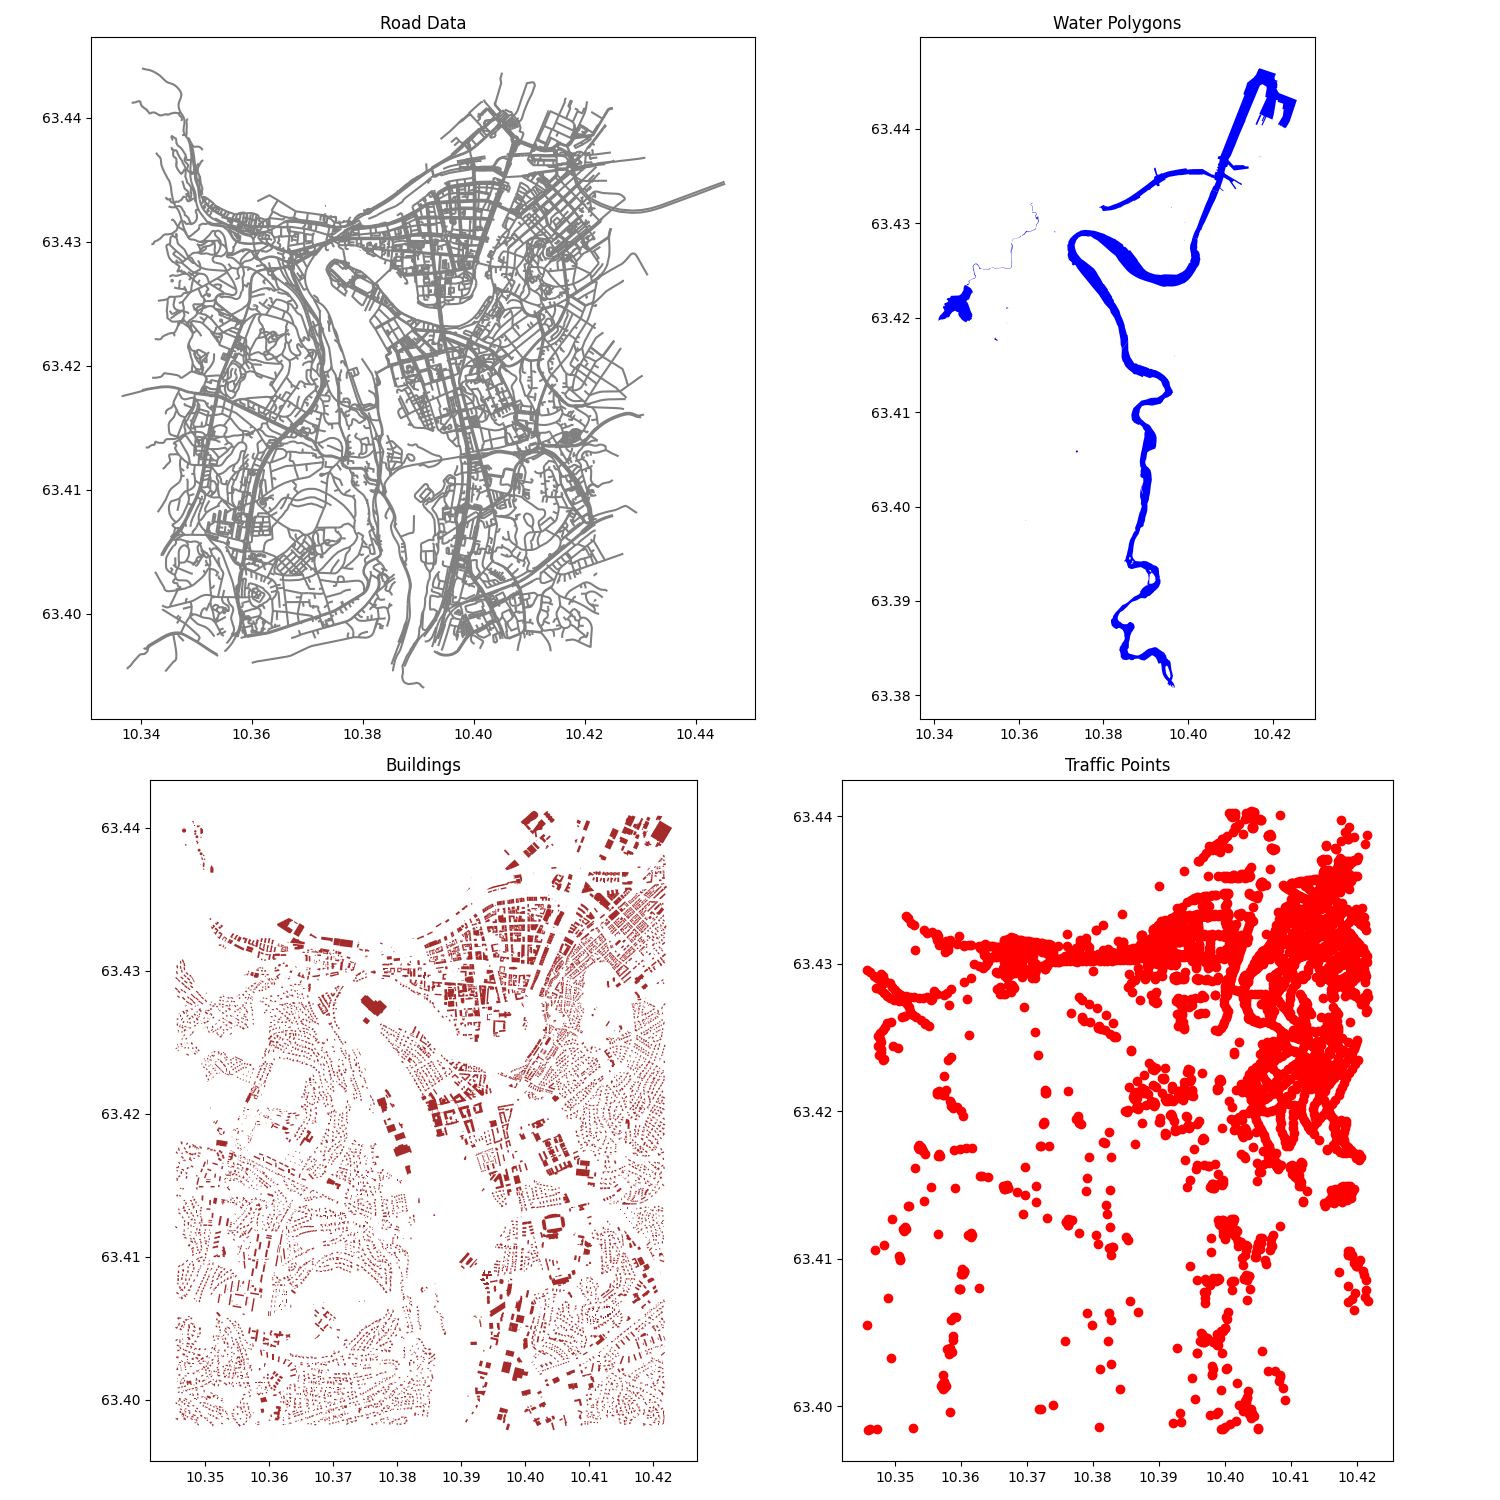
\includegraphics[width=\textwidth]{trondheim_datasets.png}
    \caption[A plot of four selected datasets constrained to a polygon of Trondheim]{A plot of four selected datasets constrained to a polygon of Trondheim. From top-left, clockwise: road lines, water polygons, traffic points, and building polygons. These plots were generated by GeoGPT.}
    \label{fig:datasets-trondheim}
\end{figure}

\FloatBarrier


\section{Experimental Results}
\label{sec:experimental-results}

\begin{comment}
Results should be clearly displayed and should provide a suitable representation of your results for the points you wish to make.
Graphs should be labelled in a legible font. If more than one result is displayed in the same graph, then these should be clearly marked.
Please choose carefully rather than presenting every result. Too much information is hard to read and often hides the key information you wish to present. Make use of statistical methods when presenting results, where possible to strengthen the results.
Further, the format of the presentation of results should be chosen based on what issues in the results you wish to highlight.
You may wish to present a subset in the experimental section and provide additional results in an appendix.
Point out specifics here but save the overall/general discussion to the Discussion chapter.
\end{comment}

\Autosubsectionref{subsec:quantitative-results} and \autoref{subsec:prompt-quality-test-results} will present the outcome of the experiments presented in \autoref{subsec:benchmarking-setup} and \autoref{subsec:prompt-quality-test-setup}, respectively. Visualizations for this section were created using Matplotlib,\footnote{\url{https://matplotlib.org/} (last visited on 2nd June 2024)} a Python library suitable for creating bar charts, box plots, etc.


\subsection[GIS Benchmark Experiment --- Results]{\acrshort{acr:gis} Benchmark --- Results}
\label{subsec:quantitative-results}

\subsubsection{Outcome Evaluation}

\autoref{fig:outcome-distribution} shows a bar charts for the outcome distribution between GeoGPT's three agents. The \acrshort{acr:ogc} \acrshort{acr:api} Features agent and the Python agent have comparable results, whereas the \acrshort{acr:sql} agent performs significantly better than the other two. The \acrshort{acr:sql} agent has a success rate of 69.4\%, while the other two share a success rate of 38.9\%. Possible reasons for this are discussed in \autoref{sec:why-sql-better} of the \nameref{cha:discussion}.

\begin{figure}[htbp]
    \centering
    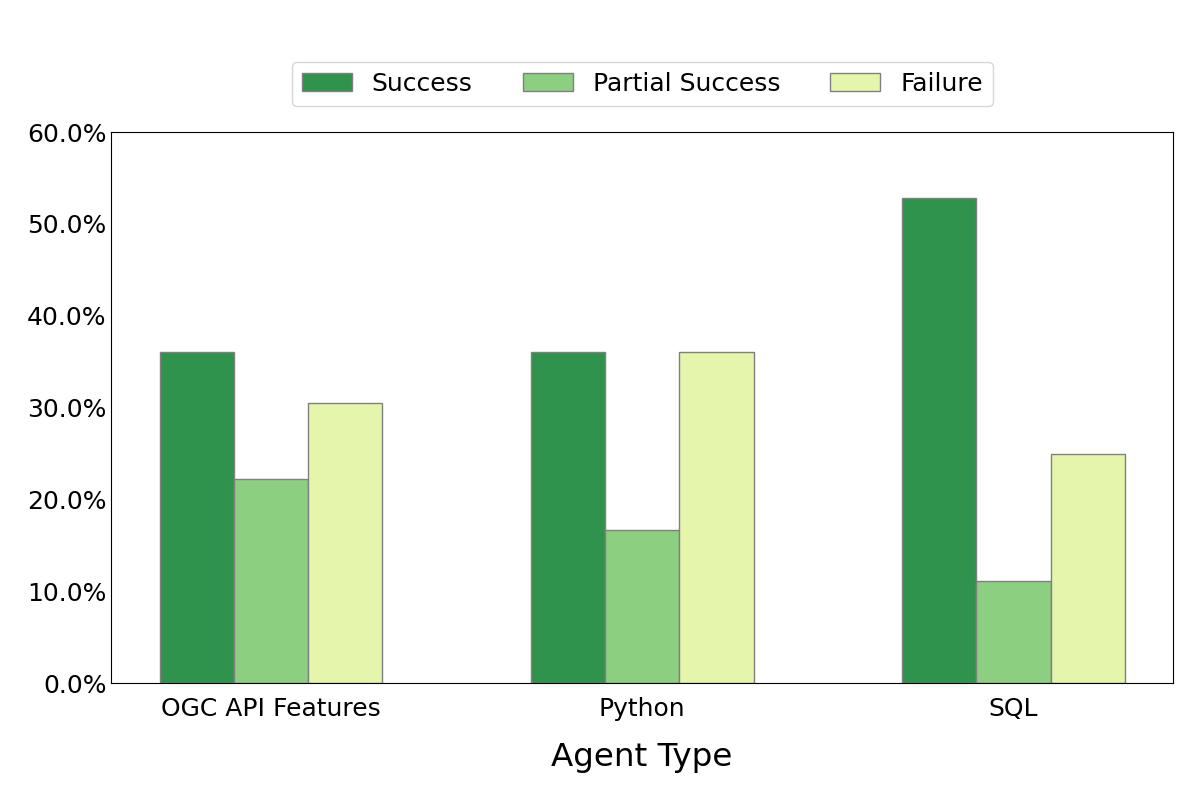
\includegraphics[width=\textwidth]{outcome_distribution_bar_chart.png}
    \caption[Outcome distribution between GeoGPT's different agent types]{Outcome distribution between GeoGPT's different agent types. The \acrshort{acr:ogc} \acrshort{acr:api} Features and Python agents perform similarly, while the \acrshort{acr:sql} agent outperforms them by a significant margin.}
    \label{fig:outcome-distribution}
\end{figure}

\subsubsection{Cost and Duration}

\autoref{fig:duration-box-plot} displays a box plot with a logarithmic y-axis that shows task durations between the different agent types. Here we can see that the \acrshort{acr:sql} agent spends the least amount of time per task. The \acrshort{acr:ogc} \acrshort{acr:api} Features agent has a slightly higher median, but with a few time-consuming outliers. The Python agent is the odd one out with a median of $\sim 82$ seconds, a $Q3 \sim 293$ seconds, and a $Q4 \sim 984$ seconds. The large gap from the Python agent to the other two agents it largely due to the Python agent's tendency to load large datasets into memory. For instance, when attempting the task of calculating the difference between the polygon outlining Oslo and water polygons (see \autoref{tbl:questions-quantitative} for the task formulation), the Python agent used nearly 40 minutes on the entire task. $94\%$ of the time was spent executing the code in \autoref{code:python-oslo-water-diff}. The main reason for the long execution time is line 8, where the whole \texttt{osm\_landuse\_polygons.shp} dataset is loaded into memory. This dataset has a size of $\sim 1.4 \text{ GB}$ and a total of 1,861,199 polygon features, and loading such amounts of data in this way is very time-consuming. The Python agent was the only agent with such issues because the \acrshort{acr:ogc} \acrshort{acr:api} Features agent is limited to 10,000 features per request, and the \acrshort{acr:sql} agent does not load the data into memory like the other agents do.

\begin{figure}[htbp]
    \centering
    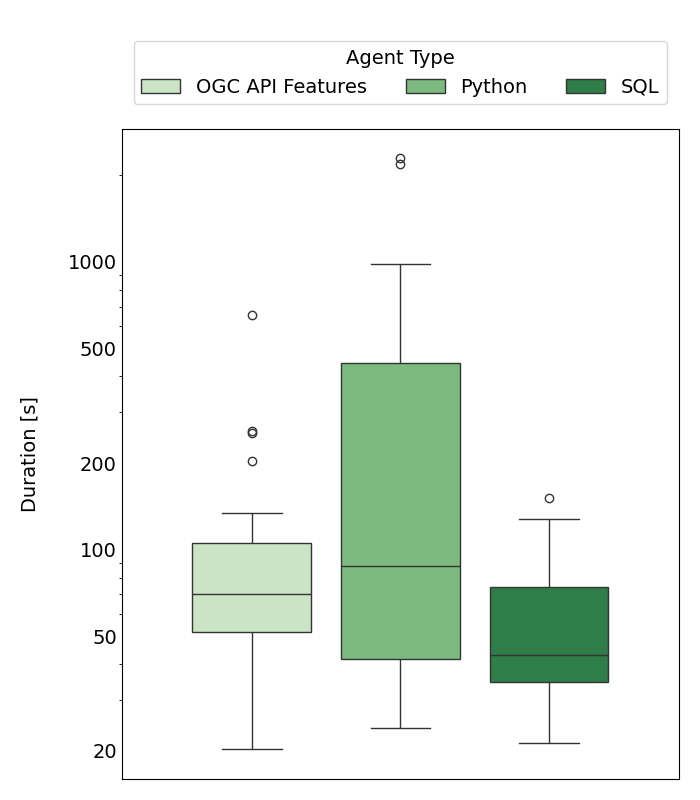
\includegraphics[width=0.6\textwidth]{duration_box_plot.png}
    \caption[Box plots comparing the time taken to generate answers between GeoGPT's agent types]{Box plots comparing the time taken to generate answers between GeoGPT's agent types. Again, the \acrshort{acr:sql} agent performs best, while the Python agent is the odd one out with very slow times compared to the other two.}
    \label{fig:duration-box-plot}
\end{figure}

\FloatBarrier

\begin{lstlisting}[
    language=Python,
    caption={[GeoGPT-generated Python code aimed at computing the difference between the outline of Oslo and residental features within it]GeoGPT-generated Python code aimed at computing the difference between the outline of Oslo, the Norwegian capital, and residental features within it. The execution time of this code block was $\sim 36$ minutes, mostly due to line 8.},
    label=code:python-oslo-water-diff,
    float
]
    import geopandas as gpd

    # Paths to the shapefiles
    landuse_path = '/tmp/tmpsutdy6it/osm_landuse_polygons.shp'
    places_path = '/tmp/tmpsutdy6it/osm_places_polygons.shp'
    
    # Load the data from shapefiles
    landuse_gdf = gpd.read_file(landuse_path)
    places_gdf = gpd.read_file(places_path)
    
    # Filter out 'residential' areas from the landuse data
    residential_gdf = landuse_gdf[landuse_gdf['fclass'] == 'residential']
     
    # Compute the spatial difference to exclude residential areas from the places data
    oslo_outline = gpd.overlay(places_gdf, residential_gdf, how='difference')
    
    # Path for the output GeoJSON file
    output_path = '/tmp/tmpsutdy6it/oslo_outline_no_residential.geojson'
    
    # Save the resulting GeoDataFrame to a GeoJSON file
    oslo_outline.to_file(output_path, driver='GeoJSON')
    
    # Output the path to the saved file
    print(output_path)    
\end{lstlisting}

\autoref{fig:cost-and-tokens} shows box plots for token usage and cost per run. Naturally, these figures appear very similar, since prices for the input tokens and generated output tokens are fixed for the models used. According to OpenAI's webpages,\footnote{\url{https://openai.com/pricing} (last visited 2nd June 2024)} they charge $\$10$ per million input tokens and $\$30$ per million output tokens for their \acrshort{acr:gpt}-4 Turbo model. From the results of the experiments, a ratio of approximately $\text{\$}10.7$ per million tokens --- either input \textit{or} output --- was calculated, which is closest to the input token price. This shows that \textit{a lot} more input tokens were used, compared to output tokens.

\begin{figure}[htbp]
    \centering
    \begin{subfigure}[b]{0.48\textwidth}
        \centering
        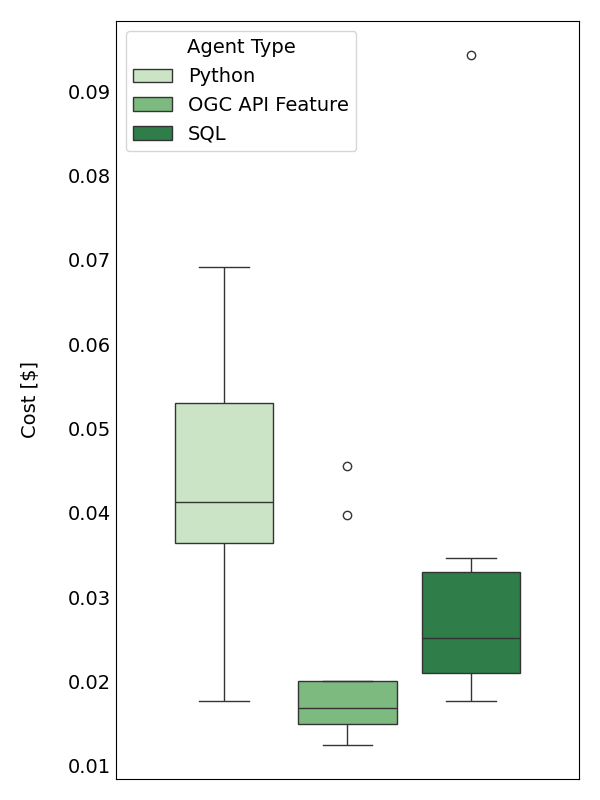
\includegraphics[width=\textwidth]{cost_box_plot.png}
        \caption{Average cost per answer between the agent types}
        \label{fig:cost-box-plot}
    \end{subfigure}
    \hfill
    \begin{subfigure}[b]{0.48\textwidth}
        \centering
        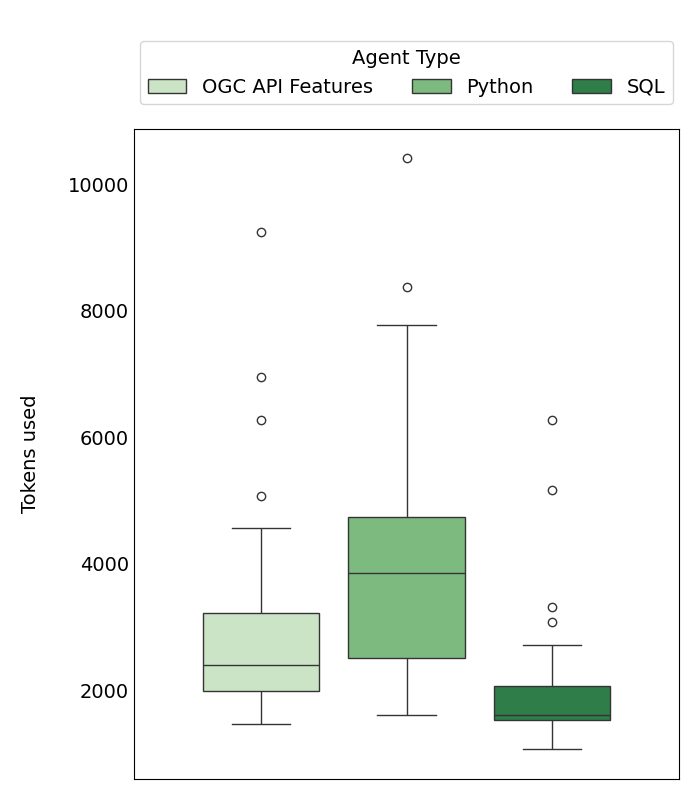
\includegraphics[width=\textwidth]{tokens_box_plot.png}
        \caption{Average token usage per answer between the agent types}
        \label{fig:tokens-box-plot}
    \end{subfigure}
    \caption[Cost and token usage between GeoGPT's different agent types]{Cost and token usage between GeoGPT's different agent types. These plots are highly correlated, but will differ somewhat because of the ratio between input and output tokens.}
    \label{fig:cost-and-tokens}
\end{figure}

An observation that can be made from the correlation matrices in \autoref{fig:correlation-matrices} is that the correlation between duration and token usage is inconsistent between the agent types. The \acrshort{acr:ogc} \acrshort{acr:api} Features agent and \acrshort{acr:sql} agent have strong correlation between these metrics, but the Python agent has next to none. This supports the observation that, for the Python agent, code execution time, particularly the time spent on expensive imports, is likely the main contributor towards the total run time.

Another observation that can be made from the \autoref{fig:correlation-matrices} is the slight negative correlation between the encoded outcome and each of the following variables: token usage, duration, and total cost. This suggests that a task that takes longer to complete, and has a higher token usage, is \textit{less} likely to produce a successful outcome. Possible reasons as to why this is the case will be explored in \autoref{subsec:dead-ends} in the \nameref{cha:discussion}.

\begin{figure}[htp]
    \centering

    \begin{subfigure}[b]{\textwidth}
        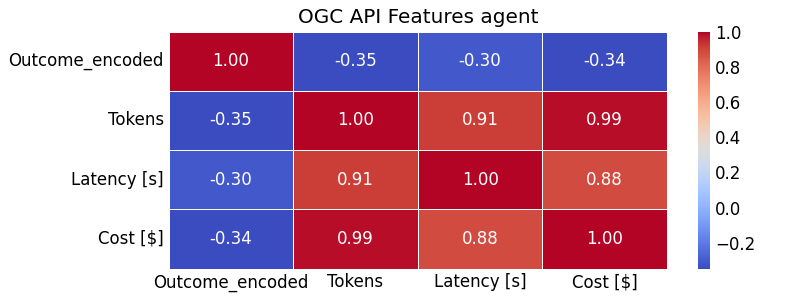
\includegraphics[width=\textwidth]{correlation_matrix_oaf.png}
        \caption{Correlation matrix for the \acrshort{acr:ogc} \acrshort{acr:api} Features agent}
        \label{fig:sub1}
    \end{subfigure}

    \vspace{1cm}

    \begin{subfigure}[b]{\textwidth}
        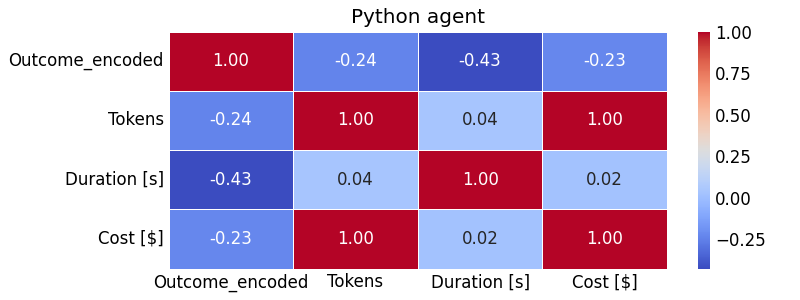
\includegraphics[width=\textwidth]{correlation_matrix_python.png}
        \caption{Correlation matrix for the Python agent}
        \label{fig:sub2}
    \end{subfigure}

    \vspace{1cm}

    \begin{subfigure}[b]{\textwidth}
        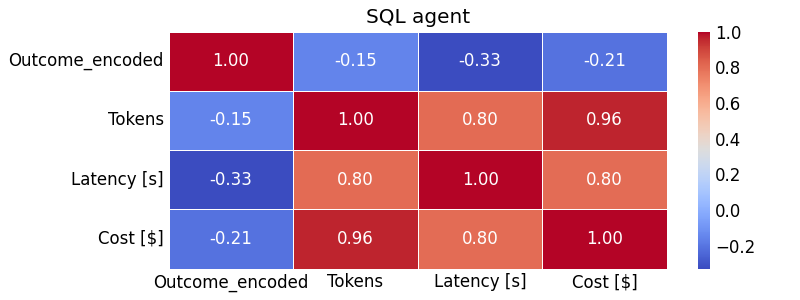
\includegraphics[width=\textwidth]{correlation_matrix_sql.png}
        \caption{Correlation matrix for the \acrshort{acr:sql} agent}
        \label{fig:sub3}
    \end{subfigure}

    \caption{Correlation matrices for the metrics recorded during the \acrshort{acr:gis} benchmark experiment for the three agent types}
    \label{fig:correlation-matrices}
\end{figure}

\subsubsection{Repeatability}

\autoref{tbl:stddev-by-agent-type} shows the average standard deviation of the outcomes for each agent type, as well as the mean of these three standard deviations. These numbers indicate that there is a notable amount of inconsistency in GeoGPT's answers when task and agent type stays the same, on average deviating with more than a third of an outcome category (0.376 for the encoded values).

\begin{table}[htbp]
    \centering
    \caption{Standard deviations of encoded outcomes for GeoGPT's agent types}
    \label{tbl:stddev-by-agent-type}
    \begin{tabularx}{0.7\textwidth}{XX}
        \toprule
        \textbf{Agent Type}                            & \textbf{Outcome Std. Deviation} \\
        \midrule
        \acrshort{acr:ogc} \acrshort{acr:api} Features & 0.552                           \\
        Python                                         & 0.337                           \\
        \acrshort{acr:sql}                             & 0.241                           \\
        \midrule
        \textbf{Mean}                                  & 0.376                           \\
        \bottomrule
    \end{tabularx}
\end{table}

\FloatBarrier

\subsubsection{Successful Responses}

% 6df94421-6c7c-470a-af8e-7013f3bc547f
\autoref{fig:glomma-counties-sql-successful} shows a successful response from GeoGPT's \acrshort{acr:sql} agent when asked how many counties the Glomma river runs through.\footnote{This run was not part of the results used for evaluation due to a bug in the \texttt{sql\_db\_query} tool that caused it to unnecessarily execute queries twice. GeoGPT's response would not be different had the bug not been present for the run, but it would have taken longer to complete.} GeoGPT correctly lists all four correct counties in a numbered list. \autoref{code:glomma-counties-sql} shows the code generated by GeoGPT for the second invocation of \texttt{sql\_db\_query}. The second invocation is nearly identical to the first one, but in the first invocation the geometry column was not included in the response, meaning GeoGPT was unable to add the results to the map. The tool informs GeoGPT about this, and the agent therefore decided to run the query again, now making sure to include the geometry column in the query result, before adding the resulting GeoJSON file to the map using the \texttt{add\_geojson\_to\_map} tool. A follow-up message instructed GeoGPT to \enquote{Add Glomma to the map}, allowing for visual verification that the answer it gave was correct.

\begin{figure}[htbp]
    \centering
    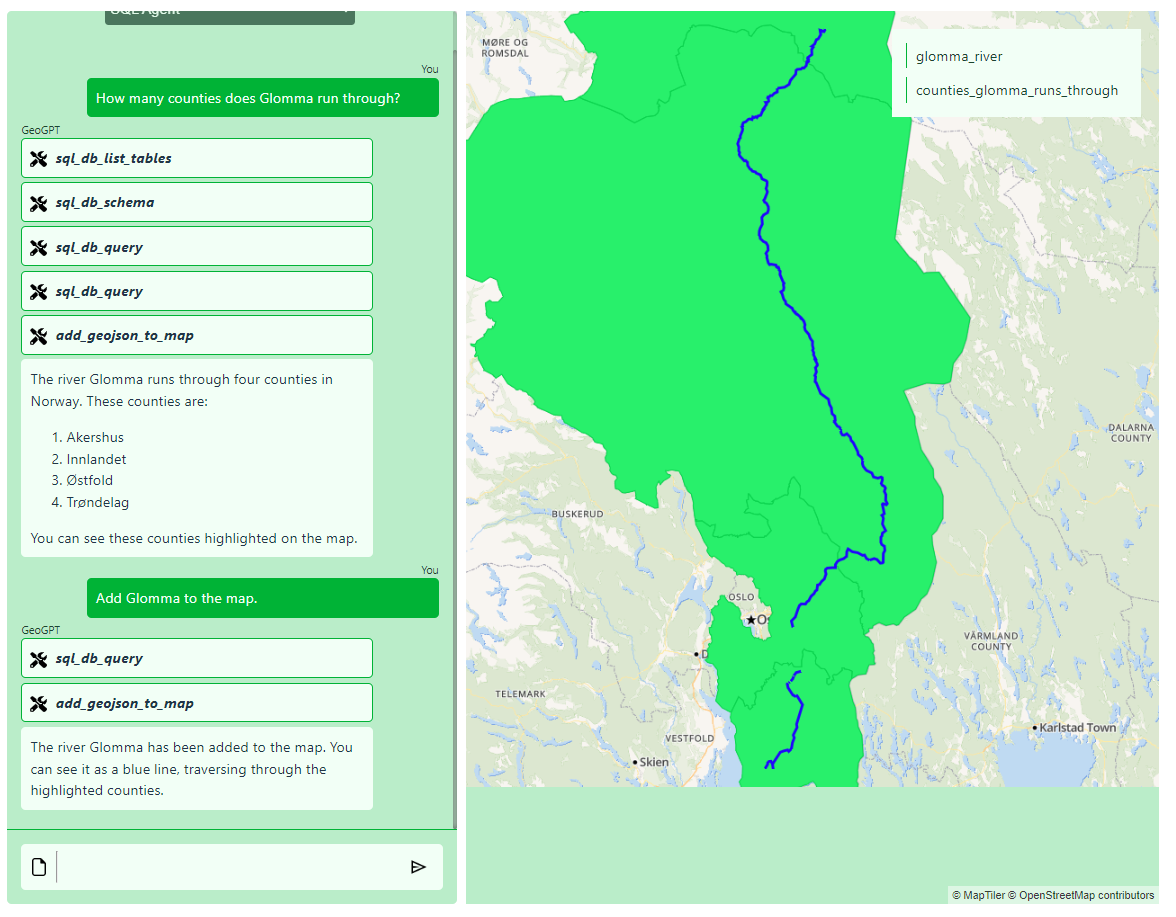
\includegraphics[width=\textwidth]{glomma_counties_sql_22.png}
    \caption[Successful response from GeoGPT's SQL agent when asked how many counties the Glomma river runs through]{Successful response from GeoGPT's \acrshort{acr:sql} agent when asked how many counties the Glomma river runs through. Using the tools available to it, GeoGPT's \acrshort{acr:sql} agent was able to to find that the river Glomma runs through the following counties: Akershus, Innlandet, Østfold, and Trøndelag. A follow-up message was added to make GeoGPT add the river geometries to the map, for verification of its results.}
    \label{fig:glomma-counties-sql-successful}
\end{figure}

\FloatBarrier

\begin{lstlisting}[
    language=sql,
    caption={[GeoGPT-generated SQL code to retrieve the counties that the Glomma river runs through]GeoGPT-generated \acrshort{acr:sql} code to retrieve the counties that the Glomma river runs through. The \texttt{ST\_Intersects} function from PostGIS was used to find the intersection between the river data and the county polygons, and the names and geometries of the counties was included in the result.},
    label=code:glomma-counties-sql,
]
WITH river AS (
    SELECT geom 
    FROM osm_waterways_lines 
    WHERE fclass = 'river' AND name ILIKE 'Glomma'
),

places AS (
    SELECT geom, name 
    FROM osm_places_polygons 
    WHERE fclass = 'county'
)

SELECT DISTINCT places.name AS county_name, places.geom AS geom
FROM river, places
WHERE ST_Intersects(river.geom, places.geom);    
\end{lstlisting}

\FloatBarrier

\autoref{fig:trees-along-munkegata-python-partial-success} shows a partially successful attempt from GeoGPT's Python agent to calculate the number of trees along Munkegata in Trondheim. While setting a definitive answer to such a question is difficult, the correct answer was set to about 100, assuming a 20-meter buffer around the line segments that make up the road. In \autoref{code:python-munkegata-bbox}, we can see how GeoGPT loads the road data around Munkegata in Trondheim, using an approximate bounding box to avoid retrieving roads named \enquote{Munkegata} in other cities. It then filters and saves the loaded data to only include features named Munkegata. In the following code block, shown in \autoref{code:python-trees-count-munkegata}, GeoGPT gets the tree data by filtering the \texttt{osm\_natural\_points} dataset on the \texttt{fclass} attribute, before loading the road data for Munkegata from \autoref{code:python-munkegata-bbox}, converting both datasets to a metric \acrshort{acr:crs}, creating a buffer around the road data, performing an intersection between the buffer, and finally printing the \texttt{tree\_count} to the standard output.

\begin{figure}[htbp]
    \centering
    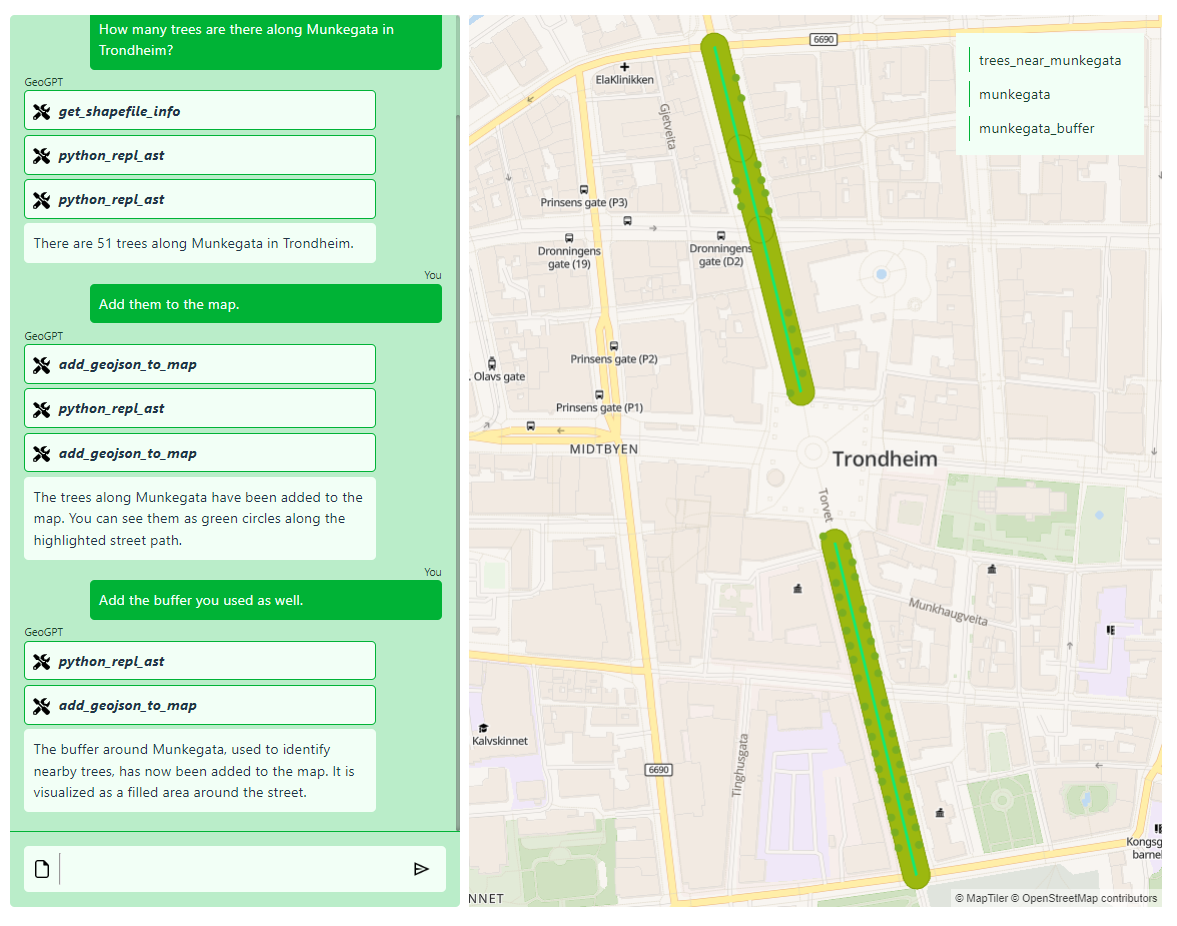
\includegraphics[width=\textwidth]{num_trees_along_munkegata_python_with_buffer.png}
    \caption[Partially successful response from GeoGPT's Python agent when asked how many trees there are along Munkegata in Trondheim]{Partially successful response from GeoGPT's Python agent when asked how many trees there are along Munkegata in Trondheim. It managed to find the road segments corresponding to Munkegata in Trondheim, but created a slightly too small buffer around it, which did not cover all the relevant trees.}
    \label{fig:trees-along-munkegata-python-partial-success}
\end{figure}

\FloatBarrier

\begin{lstlisting}[
    language=python,
    caption={[GeoGPT-generated Python code to retrieve the Munkegata road in Trondheim]GeoGPT-generated Python code to retrieve the Munkegata road in Trondheim. The bounding box, which is generated from \acrshort{acr:gpt}-4's background knowledge, covers a suitable area in the center of Trondheim, where Munkegata is located. This step is important, as a road named \enquote{Munkegata} can also be found in Oslo, which is located in a \textit{completely different} part of Norway.},
    label=code:python-munkegata-bbox,
]
import geopandas as gpd

# Load roads data with a focus on Munkegata
roads_path = '/tmp/tmpl8zsdj6m/osm_roads_lines.shp'
munkegata_bbox = (10.3910, 63.4270, 10.4030, 63.4330) # Approximate bounding box around Munkegata
munkegata_roads = gpd.read_file(roads_path, bbox=munkegata_bbox)

# Filter for Munkegata
munkegata = munkegata_roads[munkegata_roads['name'] == 'Munkegata']

# Save filtered Munkegata road to GeoJSON
munkegata_path = '/tmp/tmpl8zsdj6m/munkegata.geojson'
munkegata.to_file(munkegata_path, driver='GeoJSON')

print(munkegata_path)
\end{lstlisting}

\FloatBarrier

\begin{lstlisting}[
    language=python,
    caption={[GeoGPT-generated Python code to calculate the number of trees along Munkegata in Trondheim]Python code to calculate the number of trees along Munkegata in Trondheim. The datasets were converted to a metric \acrshort{acr:crs} (WGS 84 / UTM zone 33N), before a buffer around the road data from \autoref{code:python-munkegata-bbox} was created and used to find the intersection with the tree data. 51 trees were found, but ideally $\sim 100$ should be returned.},
    label=code:python-trees-count-munkegata,
]
from shapely.geometry import box
import geopandas as gpd

# Load the trees points
natural_points_path = '/tmp/tmpl8zsdj6m/osm_natural_points.shp'
trees = gpd.read_file(natural_points_path)

# Filter for trees
trees = trees[trees['fclass'] == 'tree']

# Load Munkegata road
munkegata_path = '/tmp/tmpl8zsdj6m/munkegata.geojson'
munkegata_road = gpd.read_file(munkegata_path)

# Project to UTM for accurate distance measurement
munkegata_utm = munkegata_road.to_crs(epsg=32633)
trees_utm = trees.to_crs(epsg=32633)

# Buffer Munkegata by 10 meters to include nearby trees
tree_buffer = munkegata_utm.buffer(10)

# Spatial join trees within buffered Munkegata
trees_near_munkegata = gpd.sjoin(trees_utm, gpd.GeoDataFrame(geometry=tree_buffer), how='inner', op='intersects')

# Count the number of trees
tree_count = trees_near_munkegata.shape[0]
print(tree_count)

# --> 51
\end{lstlisting}

\FloatBarrier
\newpage

\subsubsection{Unsuccessful Responses}
\label{subsubsec:unsuccessful-responses}

This section will highlight some limitation in the current version of GeoGPT. \autoref{fig:python-high-speed-roads-unsuccessful} illustrates an issue sometimes encountered with GeoGPT, which will be a central topic in the \nameref{cha:discussion}. Here, the Python agent has failed to recognize that the road datasets it has available is in fact for the whole of Norway, not just Oslo, the country's capital. As \autoref{code:python-high-speed-unsuccessful} shows, the agent performs the correct analysis based on the assumptions it has already made, but the answer is far from what the user enquired.

\begin{lstlisting}[
    language=python,
    caption={[GeoGPT-generated Python code that saves high-speed roads with a misleading filename]GeoGPT-generated Python code that saves high-speed roads with a misleading filename. This was the source of error that lead to the result in \autoref{fig:python-high-speed-roads-unsuccessful}. GeoGPT assumed that the \texttt{osm\_roads\_lines.shp} included road data only for \textit{Oslo}, when in reality it includes data for the \textit{whole of Norway}.},
    label=code:python-high-speed-unsuccessful,
    float
]
import geopandas as gpd

# Define the file path for the roads shapefile
shapefile_path = '/tmp/tmpr1hvr_c5/osm_roads_lines.shp'

# Read the shapefile with a condition on maxspeed being >= 70
roads_gdf = gpd.read_file(shapefile_path)
roads_high_speed_gdf = roads_gdf[roads_gdf['maxspeed'].astype(float) >= 70]

# Save the filtered GeoDataFrame as GeoJSON
output_geojson_path = '/tmp/tmpr1hvr_c5/oslo_high_speed_roads.geojson'
roads_high_speed_gdf.to_file(output_geojson_path, driver='GeoJSON')

print(output_geojson_path)
\end{lstlisting}

\FloatBarrier

\begin{figure}[htbp]
    \centering
    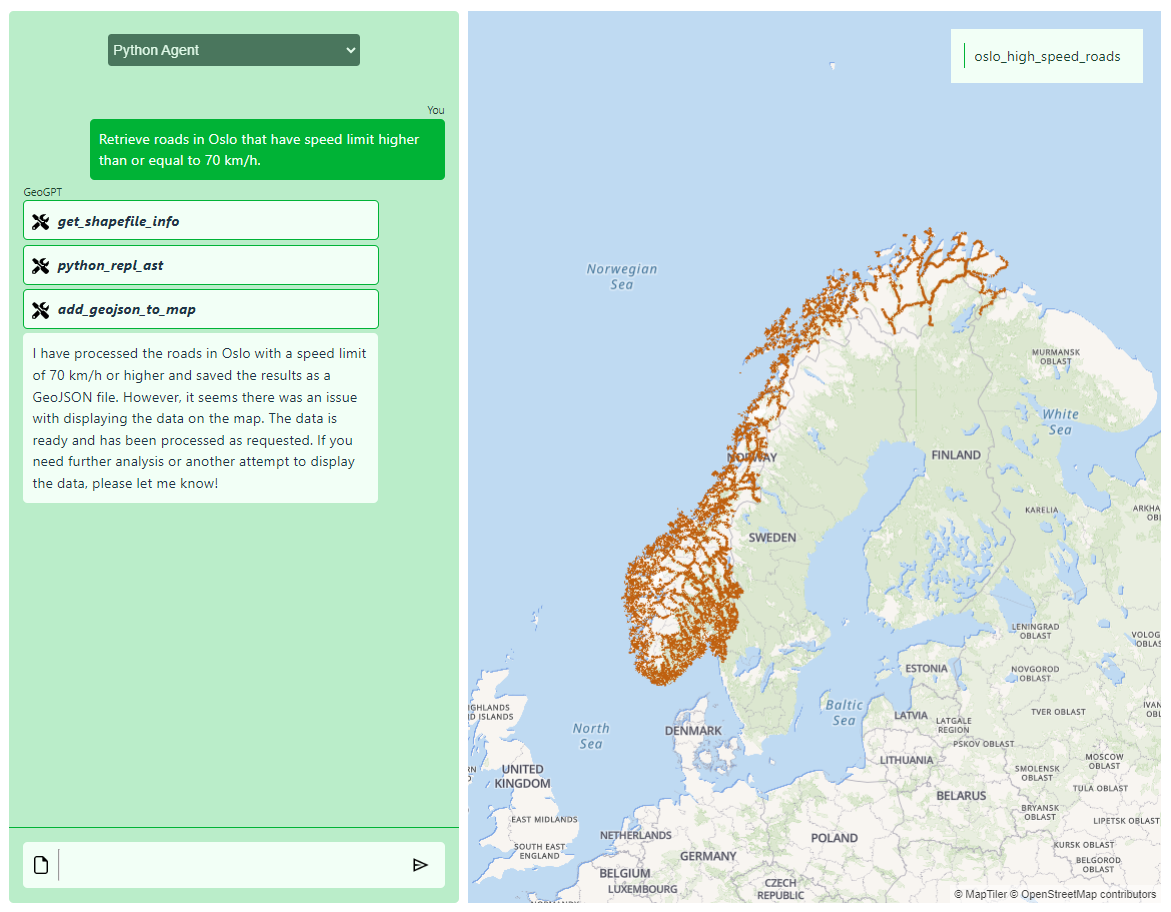
\includegraphics[width=\textwidth]{oslo_roads_maxspeed_hte_70_kmh_python.png}
    \caption[Unsuccessful attempt by GeoGPT's Python agent to retrieve high-speed roads in Oslo]{Unsuccessful attempt by GeoGPT's Python agent to retrieve high-speed roads in Oslo. The figure shows roads throughout \textit{the whole of} Norway with speed limits of 70 km/h or higher, but it should only have shown those in Oslo, the Norwegian capital.}
    \label{fig:python-high-speed-roads-unsuccessful}
\end{figure}


\FloatBarrier

\autoref{fig:oaf-geodesic-unsuccessful} shows an unsuccessful attempt from GeoGPT's \acrshort{acr:ogc} \acrshort{acr:api} Features agent to create a geodesic line between Oslo Airport Gardermoen and Bergen Airport Flesland. \autoref{code:query-collection-airports-no-results} shows GeoGPT's attempt to download a point feature with the name of \enquote{Oslo Airport}. It turns out that no such point feature exists, and only a polygonal feature in another dataset is available for the airport. The same is the case for Bergen Airport. GeoGPT made many attmpts at fetching point data for the airports, but of course none of them  returned any results.

Eventually, GeoGPT downloads a set of features from the \texttt{osm\_transport\_points} collection twice, naming them \enquote{oslo\_airport.geojson} and \enquote{bergen\_airport.geojson}. It then produces the code shown in \autoref{code:python-airports-desperate}, where it selects the first point feature in each collection and assumes that their coordinates correspond to Oslo and Bergen. These two features actually correspond to are Rakkestad Airport and a bus stop on a road along Ofotfjorden in Nordland. In addition to this mistake, subsequent attempts at creating a geodesic line between the locations were unsuccessful.

\begin{figure}[htbp]
    \centering
    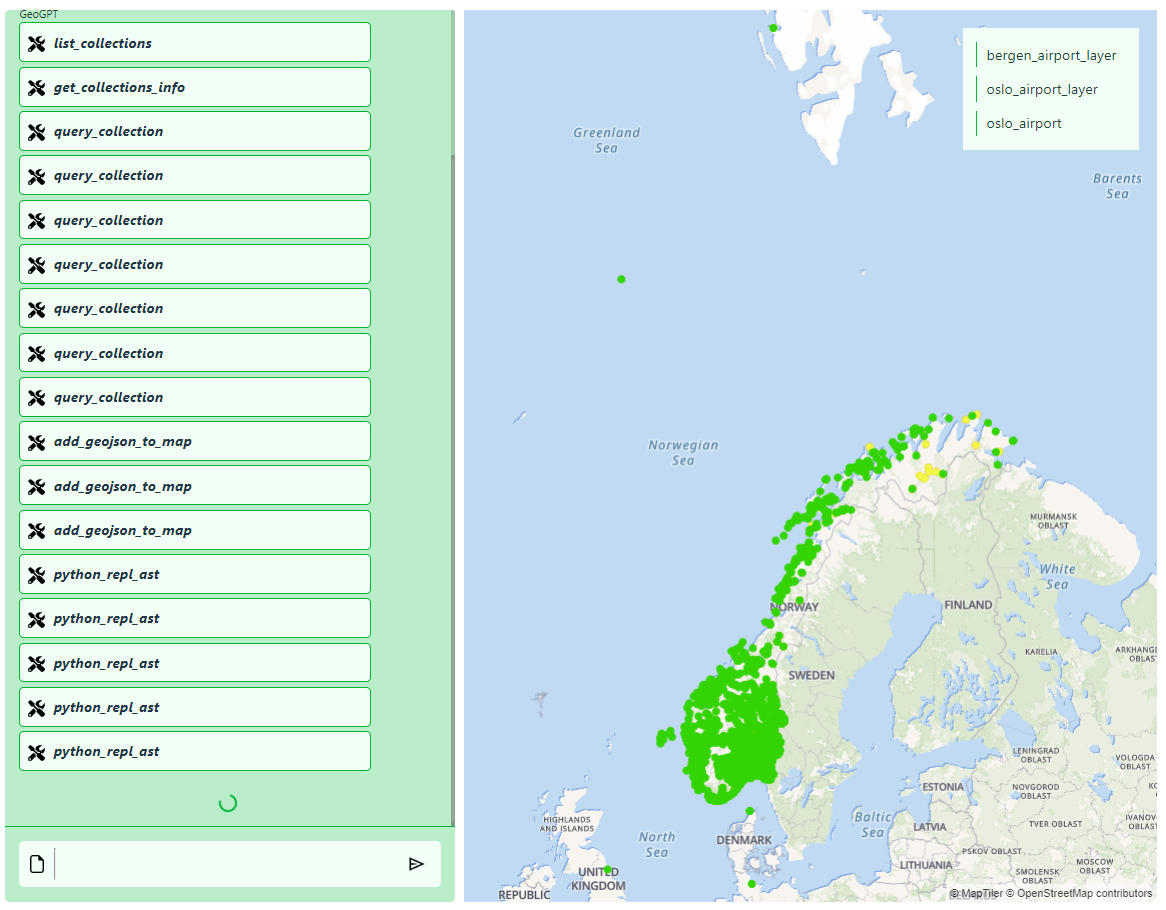
\includegraphics[width=\textwidth]{oslo_bergen_geodesic_oaf2.png}
    \caption[Unsuccessful attempt by GeoGPT's OGC API Features agent to create a geodesic line between Oslo Airport Gardermoen and Bergen Airport Flesland]{Unsuccessful attempt by GeoGPT's \acrshort{acr:ogc} \acrshort{acr:api} Features agent to create a geodesic line between Oslo Airport Gardermoen and Bergen Airport Flesland. GeoGPT has added datasets, assuming they contain airport point data, when in reality they contain traffic point data for the whole of Norway. The result should have been a geodesic line between Gardermoen (in the south-east of Norway) and Flesland (in the south-west of Norway).}
    \label{fig:oaf-geodesic-unsuccessful}
\end{figure}

% \FloatBarrier

\begin{lstlisting}[
    language=json,
    caption={[Invocation of the \texttt{query\_collection} tool that returned no features]Invocation of the \texttt{query\_collection} tool that returned no features. This is because there are no features named \enquote{Oslo Airport} in the \texttt{public.osm\_transport\_points} collection. The \acrshort{acr:json} object contains the parameters sent to the tool, and the text after the \enquote{\texttt{-->}} is the message returned from the tool.},
    label=code:query-collection-airports-no-results,
    float, floatplacement=H
]
{
  "collection_name": "public.osm_transport_points",
  "cql_filter": "fclass='airport' AND name='Oslo Airport'",
  "layer_name": "oslo_airport"
}

--> No features were found at http://localhost:9001/collections/public.osm_transport_points/items?limit=10000&filter=fclass='airport' AND name='Oslo Airport'.
Try to change the parameters, or make them less restrictive.
\end{lstlisting}

\FloatBarrier

\begin{lstlisting}[
    language=python,
    caption={[Unsuccessful attempt at retrieving point data for Gardermoen and Flesland]GeoGPT-generated Python code that picks the first features two collections including various point data in the \textit{hope} that they correcspond to Gardermoen and Flesland. This attempt was of course insuccessful},
    label=code:python-airports-desperate,
]
import geopandas as gpd

oslo = gpd.read_file('/tmp/tmpwlojm_1k/oslo_airport.geojson')
bergen = gpd.read_file('/tmp/tmpwlojm_1k/bergen_airport.geojson')

oslo_coords = oslo.geometry[0].coords[0]
bergen_coords = bergen.geometry[0].coords[0]

oslo_coords, bergen_coords   

# --> ((11.3469259, 59.397229), (16.919517, 68.3459))
\end{lstlisting}

% \FloatBarrier

\newpage

\subsection{Prompt Quality Experiment --- Results}
\label{subsec:prompt-quality-test-results}

\autoref{fig:outcome-distribution-experience-levels} shows the outcomes of the experiments where the importance of the quality of the user's initial prompt was evaluated. It is clear to see that \textit{expert}-level prompting significantly outperforms \textit{novice}-level prompting, the latter of which failed to produce fully responses. It is worth noting, however, that the questions picked were the three hardest ones from the \acrshort{acr:gis} benchmark experiment.

\begin{figure}[htbp]
    \centering
    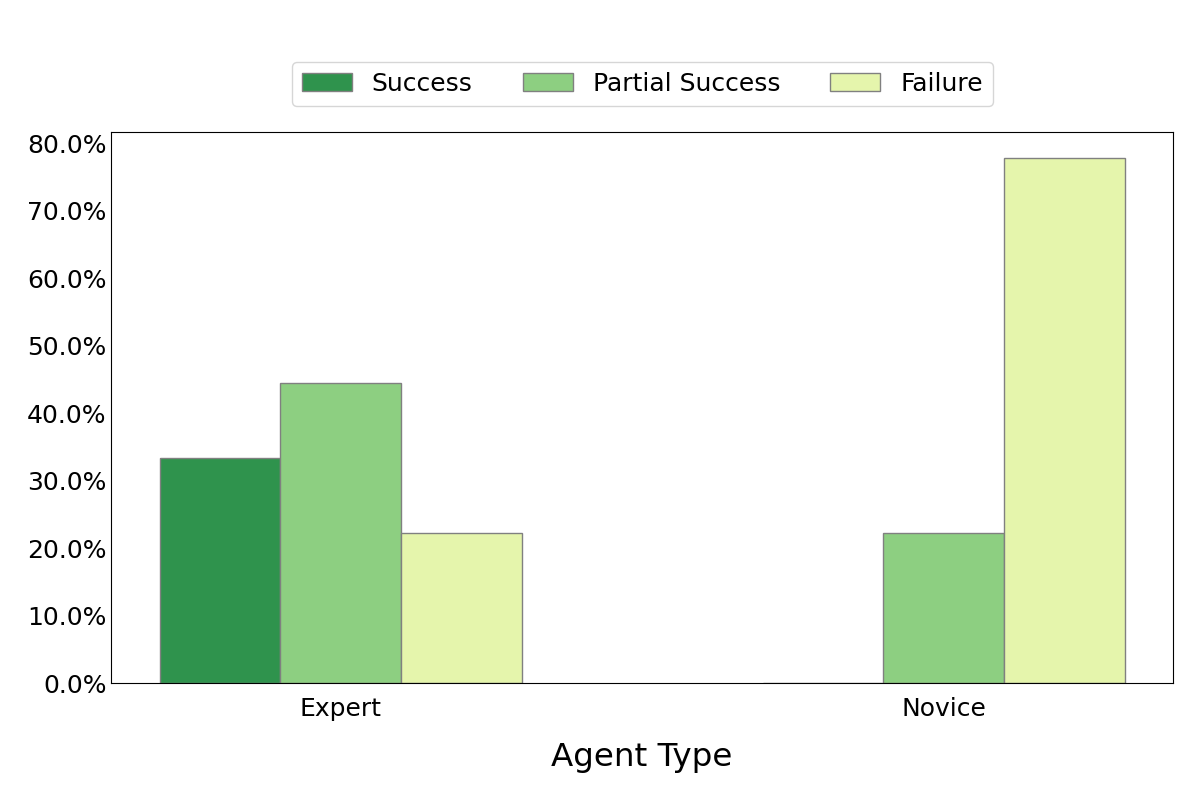
\includegraphics[width=\textwidth]{levels_outcome_distribution_bar_chart.png}
    \caption[Outcome distribution for different levels of prompt quality]{Outcome distribution for different levels of prompt quality. Using novice-level prompting, GeoGPT failed to complete the tasks consistently, but using the more elaborate expert-level prompt, GeoGPT performed much better.}
    \label{fig:outcome-distribution-experience-levels}
\end{figure}

\autoref{fig:novice-vs-expert-munkegata-trees} compares the responses that GeoGPT's \acrshort{acr:ogc} \acrshort{acr:api} Features agent managed to produce for the different prompt levels on the task of counting the number of trees along the road named \enquote{Munkegata} in Trondheim (see \autoref{tbl:questions-quantitative}). The \textit{novice}-level prompt reads as follows:

\begin{quote}
    \enquote{Could you count how many trees there are on Munkegata street in Trondheim?}
\end{quote}

\noindent The \textit{expert}-level prompt included a series of instructions:

\begin{quote}
    \enquote{1. List all datasets that could possibly include trees. \\
        2. Find the correct feature class and filter the relevant dataset to access tree data for Trondheim. Use a bounding box to reduce the number of trees to analyse. \\
        4. Fetch road data for Munkegata. Use a bounding box for Trondheim in case there are streets elsewhere named Munkegata. \\
        5. Convert both datasets to a suitable metric CRS and add a 20-meter buffer around the road data. \\
        6. Find all trees that lie within this buffer and count them. \\
        7. Present the findings with a map highlighting the roads and the trees.}
\end{quote}

\FloatBarrier

When using the novice-level prompt, GeoGPT was unable to produce the correct outcome, and confidently answered that there are \enquote{approximately 6,915 trees on Munkegata street in Trondheim}, which is far from being true. When solving the task, GeoGPT made a series of oversights that lead to this result. First, it failed to take into account that there may be more than one street in the dataset named \enquote{Munkegata}, missing the important step of applying a bounding box filter to the query. A similar mistake was made when retrieving the tree data. Due to the upper limit of 10,000 features per request to the \acrshort{acr:ogc} \acrshort{acr:api} Features server, it's crucial to narrow down the query to ensure that all relevant features are retrieved, rather than just a subset of them. GeoGPT's request lacked a bounding box, resulting in a randomly distributed subset of 10,000 trees, scattered across the whole of Norway. A third mistake occurred when GeoGPT calculated a bounding box around the retrieved road data instead of creating a buffer. Using a buffer would have produced a more accurate result. The bounding box that was created spanned from Trondheim to Oslo, thus including far more trees than was intended.

The expert-level prompt, on the other hand, provided the necessary guidance for GeoGPT for this specific task, steering it clear of the issues it encountered with the novice-level prompt. As OpenAI themselves stated, \enquote{some tasks are best specified as a sequence of steps}.\footnote{\url{https://platform.openai.com/docs/guides/prompt-engineering/strategy-write-clear-instructions} (last visited 2nd June 2024)} Furthermore, they say that writing explicit steps required to solve a task \enquote{makes it easier for the model to follow them}.

\begin{figure}[htbp]
    \centering
    \begin{subfigure}[b]{0.7\textwidth}
        \centering
        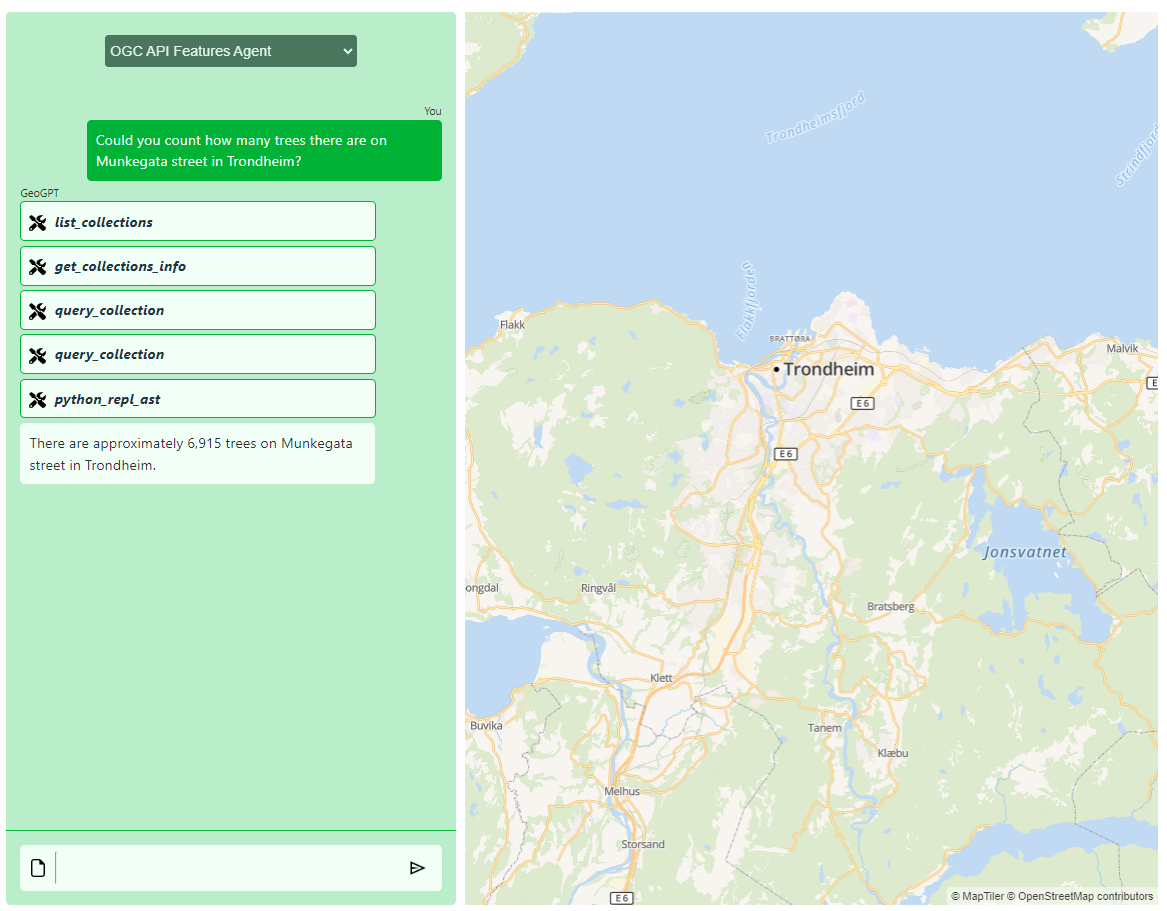
\includegraphics[width=\textwidth]{munkegata_trees_oaf_novice.png}
        \caption{Novice-level prompting}
        \label{fig:novice-level-prompting-munkegata-trees}
    \end{subfigure}
    \hfill
    \begin{subfigure}[b]{0.7\textwidth}
        \centering
        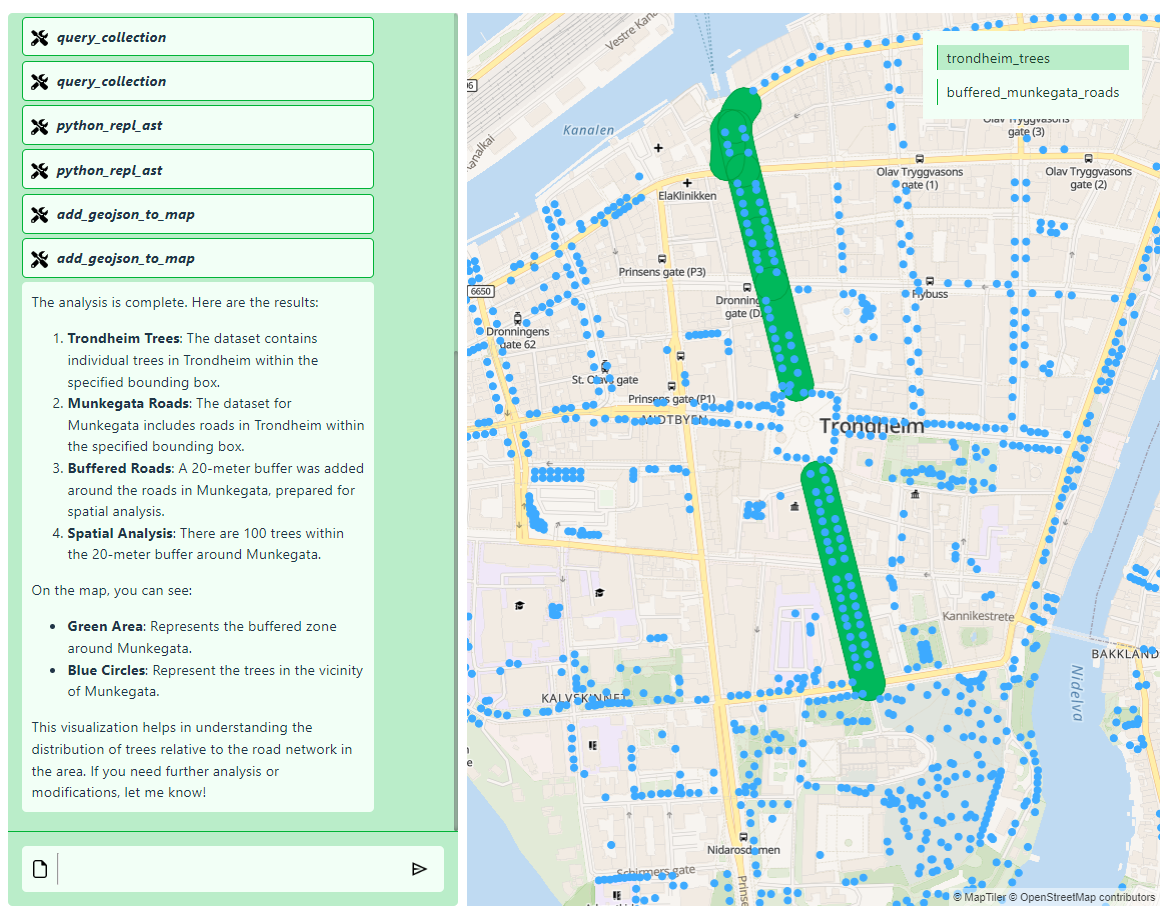
\includegraphics[width=\textwidth]{munkegata_trees_oaf_expert_sbs_2.png}
        \caption{Expert-level prompting}
        \label{fig:expert-level-prompting-munkegata-trees}
    \end{subfigure}
    \caption[Comparison between novice- and expert-level prompting of GeoGPT for calculating the number of trees along Munkegata in Trondheim.]{Comparison between novice- and expert-level prompting of GeoGPT's \acrshort{acr:ogc} \acrshort{acr:api} Features on the task of calculating of the number of trees along Munkegata in Trondheim. Using the novice-level prompt, GeoGPT found 6,915 trees (far too many). However, using the expert-level prompt, it was able to find the correct number of trees and add the appropriate layers to the map.
    }
    \label{fig:novice-vs-expert-munkegata-trees}
\end{figure}

% \begin{figure}[htbp]
%     \centering
%     \begin{subfigure}[b]{0.7\textwidth}
%         \centering
%         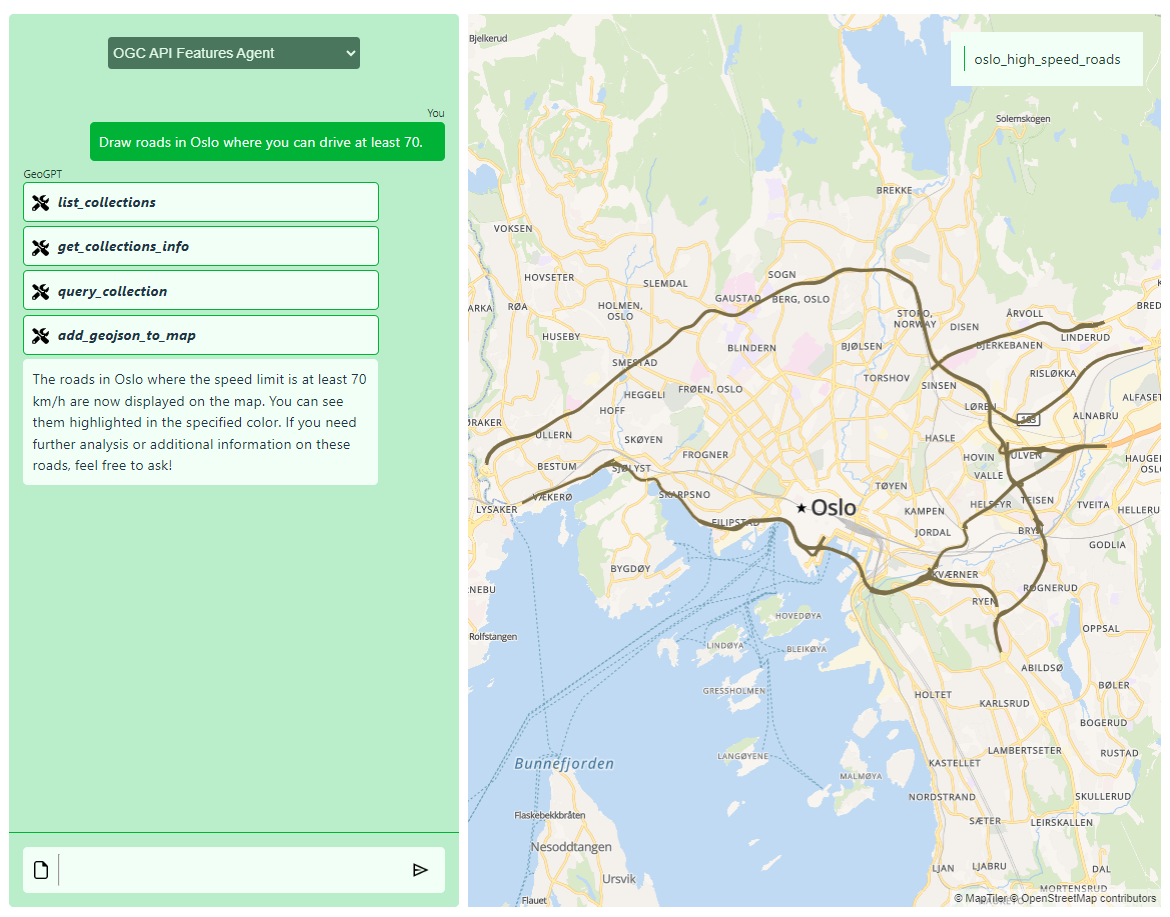
\includegraphics[width=\textwidth]{oslo_70kmh_oaf_novice.png}
%         \caption{Novice-level prompting}
%         \label{fig:novice-level-prompting-oslo-70kmh}
%     \end{subfigure}
%     \hfill
%     \begin{subfigure}[b]{0.7\textwidth}
%         \centering
%         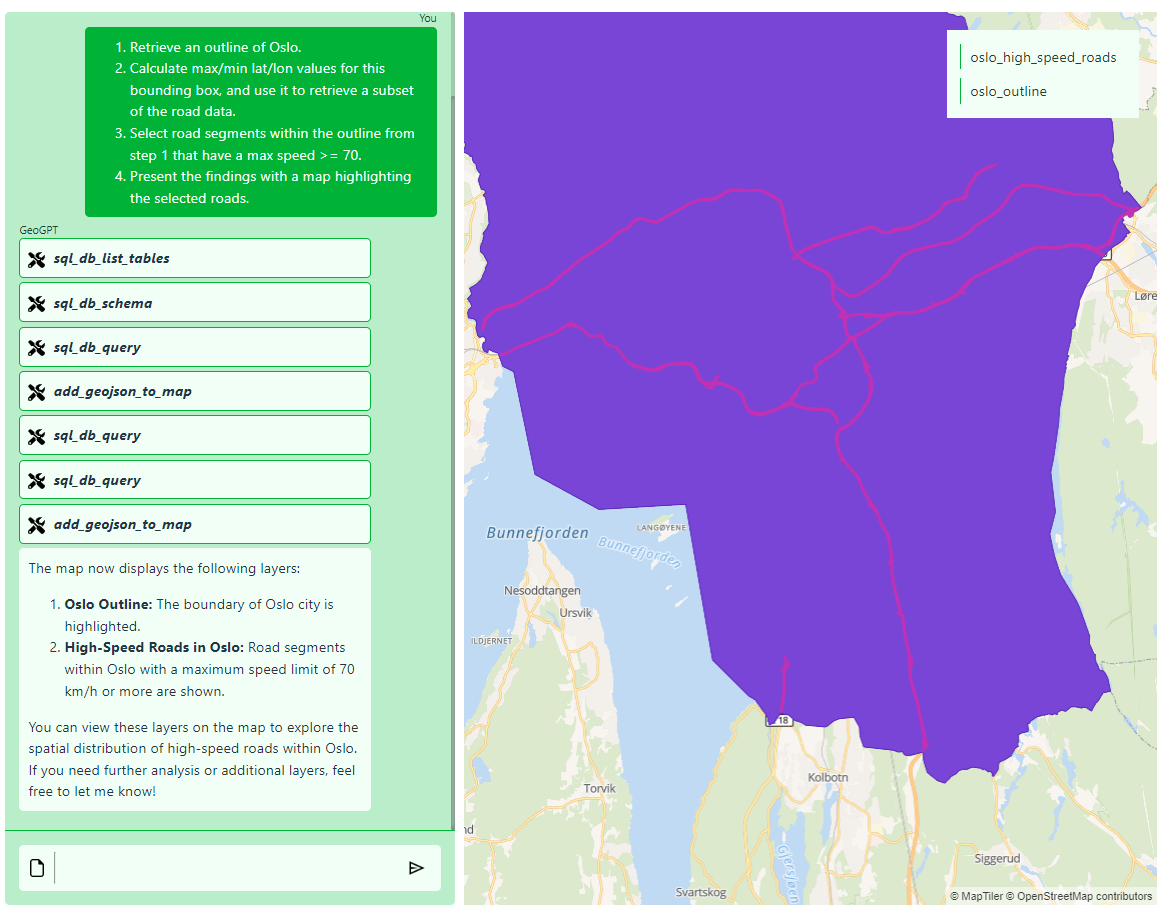
\includegraphics[width=\textwidth]{oslo_70kmh_sql_expert_sbs_2.png}
%         \caption{Expert-level prompting}
%         \label{fig:expert-level-prompting-oslo-70kmh}
%     \end{subfigure}
%     \caption{Comparison between novice- and expert-level prompting of \acrshort{acr:ogc} \acrshort{acr:api} Features agent for retrieval of high-speed roads in Oslo}
%     \label{fig:novice-vs-expert-oslo-70kmh}
% \end{figure}

\glsresetall
\chapter{Discussion and Conclusion}\label{cha:discussion-and-conclusion}

Sections \ref{sec:code-interpreter-discussion} and \ref{sec:api-access-discussion} will discuss the test results from \autoref{sec:experimental-results} and provide suggestions as to how the limitations highlighted by the tests can be mitigated. \Autosectionref{sec:conclusion-and-future-work} will conclude this specialization project report, and provide directives for future work on the subject of \acrshort{acr:llm}-powered \acrshort{acr:gis}.

\section{Using ChatGPT's Code Interpreter for Geospatial Analysis}\label{sec:code-interpreter-discussion}

When using ChatGPT's built-in Code Interpreter with file uploads, it became apparent that it runs in a Linux environment and utilizes a mounted drive in the \texttt{/mnt} directory, typically used for temporarily mounted filesystems. In an initial test on the \acrshort{acr:sosi} data format, it tried to execute this \acrshort{acr:gdal} command

$$
    \texttt{ogr2ogr -f "GeoJSON" \{converted\_geojson\_path\} \{sosi\_file\_path\}}
$$

\noindent to perform a conversion from \acrshort{acr:sosi} to GeoJSON, the latter of which is far easier to manipulate in a Python environment. This test failed, and the system's response was that \enquote{the \texttt{ogr2ogr} tool is not available in this environment}.

This result was not very surprising, especially since the driver needed to read and write \acrshort{acr:sosi} files---which is called \textit{fyba}\footnote{\url{https://github.com/kartverket/fyba}} and is developed by the Norwegian Mapping Authority---is almost certainly not available in the standard Linux environment used for ChatGPT's Code Interpreter. As the \acrshort{acr:sosi} standard is still widely used for Norwegian geospatial purposes (though according to its Wikipedia page\footnote{\url{https://no.wikipedia.org/wiki/SOSI-formatet}} expected to be exchanged with the \acrshort{acr:gml} format in the future), it is important for an \acrshort{acr:llm}-based \acrshort{acr:gis} agent focused on the Norwegian market to be able to handle this file type.

The inability of flexibly manipulating the Linux environment used by the Code Interpreter then clearly poses some limitations when developing \acrshort{acr:llm}-based systems. A possible solution is to create a custom environment on a server that we control ourselves. Having the \acrshort{acr:ai} agent run in an environment that we have full control over, gives us greater flexibility, and we can then grant the agent access to powerful \acrshort{acr:gis} tooling, such as the \acrshort{acr:gdal} library. The open-source \enquote{Open Interpreter} project \citep{killianlucasKillianLucasOpeninterpreter2023} could prove useful as an alternative to the closed-source Code Interpreter from OpenAI. Open Interpreter lets us run the interpreter on the computer/server of our choosing, so that it can access the file system directly, as well as libraries and programs stored on the computer/server. It also allows for other \acrshortpl{acr:llm} than \acrshort{acr:gpt}-4, such as Mistral \acrshortpl{acr:llm} and Code-LLaMA. Additionally, with it being an open-source project, one can \enquote{fork} the repository and make project-specific modifications to the interpreter.

\section[Mitigating ChatGPT's Inability to Access Web APIs]{Mitigating ChatGPT's Inability to Access Web \acrshort{acr:api}s}\label{sec:api-access-discussion}

As the results from Test 2 (see \autoref{subsec:experiment-2-results}) show, ChatGPT-4 struggles when provided with URLs to external web \acrshortpl{acr:api}, even when prompted to use its web browsing capabilities and pairing them with its Code Interpreter. These issues are not present when using direct file upload, in which case the model appears to save the uploaded file in a temporary file directory in its Linux environment. Interpreting the inner workings of the Code Interpreter from the code samples in the chat can be challenging, but it appears that it does not do this by default after fetching data from an external web \acrshort{acr:api}. As \autoref{lst:python-for-failed-drammen-outline} shows, it \textit{truncates} the file contents and \enquote{stores} them directly in the code, in an attempt to keep the entire file contents within the context window of the \acrshort{acr:llm}. The context window of the ChatGPT-4 model is currently at 32,000 tokens, and the new GPT-4 Turbo has a context length of 128,000 tokens. While these are of significant size, they are not meant to (or able to) store large file. The size of the context window therefore becomes a limiting factor when the file contents grow large, which is not uncommon for geospatial files.

This is a significant limitation of using ChatGPT-4 out of the box, and one should therefore look into other ways of handling web requests and subsequent storing of the received data. Techniques within \gls{acr:rag}, and libraries like LangChain and Open Interpreter, could help solve this issue.

\glsresetall

\section{Conclusion and Future Work}\label{sec:conclusion-and-future-work}

This specialization project report has presented a literature study in the fields of \acrlong{acr:nlp}, \acrlongpl{acr:llm}, \acrshort{acr:gis}, planning for \acrshortpl{acr:llm}, and \acrlong{acr:rag}, along with three tests that try to demonstrate strengths and weaknesses of \acrshortpl{acr:llm} when dealing with geospatial data. The literature study and tests serve to provide a better starting point when attempting to develop \acrshort{acr:llm}-based \acrshort{acr:gis} agents.

One important finding of the literature study is that there has been a substantial body of work done concerning the potential of using \acrlongpl{acr:llm} in \acrshort{acr:gis} analysis (see \autoref{sec:gis-with-llms}). Studies have been conducted to show that the \acrshort{acr:gpt}-4 model has good geospatial awareness, and there have been created a number of prototypes of autonomous \acrshort{acr:gis} systems powered by \acrshortpl{acr:llm}. \Autosectionref{sec:planning-strategies} discussed various planning strategies that have been developed to facilitate better decision-making and reasoning in \acrshort{acr:llm}-based systems. \Autosectionref{sec:retrieval-automented-generation} introduced \gls{acr:rag}, the concept of providing \acrshortpl{acr:llm} with access to external tooling to help them produce informed and up-to-date responses.

The three tests showcased \acrshort{acr:gpt}-4's abilities of handling geospatial data using various data formats and access channels. The results from Test 1 and 2 showed that it has \textit{some} understanding of how to perform geospatial analysis, but that it also has substantial limitations, e.g., reading and writing large files and accessing data through web \acrshortpl{acr:api}. Test 3 (see \autoref{subsec:ex-3-setup}) served as an initial test of utilizing tools such as LangChain to extend the capabilities of \acrshortpl{acr:llm} like \acrshort{acr:gpt}-4 through programmatic methods.

With this being a specialization project that will transition into a larger master thesis, some points of discussion have been reserved for future work. Additionally, the task of developing a proof of concept has been assigned to the master thesis due to time constraints and the intention to acquire more knowledge before proceeding with development. Subsections \ref{subsec:memory-and-embeddings} and \ref{subsec:testing-regime} will elaborate upon potentially important issues that should be addressed when developing \acrshort{acr:llm}-based \acrshort{acr:gis} agents.

% \subsection{Balancing Accuracy Against Performance and Costs}

% The ecosystem of agent frameworks and planning strategies to improve agent performance on complex tasks (discussed in \nameref{cha:related-work}), is a growing one. Different agents frameworks and planning strategies should be compared to see which are most viable for \acrshort{acr:gis} work. Important considerations are the ability to destructure complex problems, the ability to take advantage of external tooling, and computational time. More complex planning strategies typically demand more interactions with \acrshort{acr:llm} \acrshortpl{acr:api}, which can be expensive both in terms of computational time and cost (when using a monetized \acrshort{acr:api} like OpenAI's for \acrshort{acr:gpt}-4 and \acrshort{acr:gpt}-4).

% \cite{clearyLatencyBenchmarksComparisons2023} did benchmarking of different \acrshortpl{acr:llm} on different providers. Important takeaways were that \acrshort{acr:gpt}-4 is about 6.3 times slower than \acrshort{acr:gpt}-3.5-Instruct, and that Azure has far lower latency in most cases for inference on \acrshort{acr:gpt} models. Such considerations are important when addressing usability of \acrshort{acr:llm}-based applications, balancing accuracy against speed and cost. Using free open-source alternatives where possible is a good option to reduce cost. Open-source software like the Open Interpreter project should also be investigated.

\subsection{Memory and Embeddings}\label{subsec:memory-and-embeddings}

Storing information for future use is important when developing \acrshort{acr:llm}-based agents in order for them to produce consistent responses. \cite{wengLLMPoweredAutonomous2023} presents three different types of memory in human brains: (1) \textit{Sensory Memory}, (2) \textit{Short-Term Memory}, and (3) \textit{Long-Term Memory}. When translated to \acrshortpl{acr:llm}, we can think of \textit{Sensory Memory} as learning embedding representations, \textit{Short-Term Memory} as the memory contained within the limits of the context window of the Transformer, and  \textit{Long-Term Memory} as an external vector store that can be attended to by the agent at query time. Such a vector store/database would store the vector embeddings of the data contained within it, and allow for fast and accurate similarity search and retrieval based on the vector distance or similarity between the vector representations \citep{evchakiVectorDatabase2023}. \cite{wengLLMPoweredAutonomous2023} lists some common approximate nearest neighbours algorithms for fast retrieval speeds, including \gls{acr:lsh} and \gls{acr:faiss}.

Future work should build upon the research of \cite{unluChatmapLargeLanguage2023} (see \autoref{sec:gis-with-llms}) and investigate whether vector embeddings can be utilized for long-term storage of geospatial data with textual descriptions, or if a vector database can efficiently retrieve relevant resources such as \acrshortpl{acr:api} or other external tools based on their documentation/specifications. Furthermore, these documentations and \acrshort{acr:api} specifications can be large is size, and the context length could become a limiting issue. Vector embeddings can help mitigate such issues. By splitting the documents into chunks and indexing them using vector embeddings, one can extract only the relevant parts and pass these to the \acrshort{acr:llm} with the prompt.

\subsection{Testing Regime}\label{subsec:testing-regime}

In order to test the feasibility of different language models to serve as the brain of an autonomous \acrshort{acr:gis} agent, a testing regime should be developed. In the examples of autonomous \acrshort{acr:gis} agents described in the literature study of this report (see \autoref{sec:gis-with-llms}), results were generally presented in the form of case studies. This type of qualitative testing is entirely appropriate for showcasing the possibilities of the technologies, but it may be insufficient for comparing the performance of \textit{different} systems. A quantitative approach would probably be preferable.

One idea is to create a test dataset which consists of inputs and corresponding desired outputs of typical \acrshort{acr:gis} tasks. Inputs would in this case be natural language queries inputted by a mock user, and the outputs would be what you would expect a \acrshort{acr:gis} professional to return when given the same tasks/queries. Inputs should reflect the varying level of \acrshort{acr:gis} knowledge between different user groups (see \autoref{sec:user-groups}). Outputs could be files with typical geospatial extensions (.shp, .geojson, .sos, etc.), or they could adhere to API specifications from geospatial standards (see \autoref{sec:geospatial-standards}).

While the inputs should be fairly simple to construct, there are several questions to be answered in regard to the outputs, among which are the following:

\begin{itemize}
    \item How does one evaluate the accuracy of the output?
    \item How should the \acrshort{acr:ai} agent respond when the user does not specify an output file format?
    \item How does one evaluate the usefulness of responses to questions that should \textit{not} return geospatial files, e.g., answers to general questions about geo-related subjects?
\end{itemize}

\noindent These questions are outside the scope of this specialization project, and are therefore left out for future work.



\glsaddall

%%%%%%%%%%%%%%%%%%%%%%%%%%%%%%%%%%%%%%%%%%%%%%%%%%%%%
%\backmatter
\clearpage
\phantomsection
\addcontentsline{toc}{chapter}{Bibliography}
\printbibliography

\begin{appendix}
    \chapter*{Appendices}
    \label{cha:appendices}
    \addcontentsline{toc}{chapter}{Appendices}

    \includeappendixpdfwithtitle{Task Description from Norkart}{appendices/project_description.pdf}{app:task-description}

    % \newgeometry{top=.5in}
    % 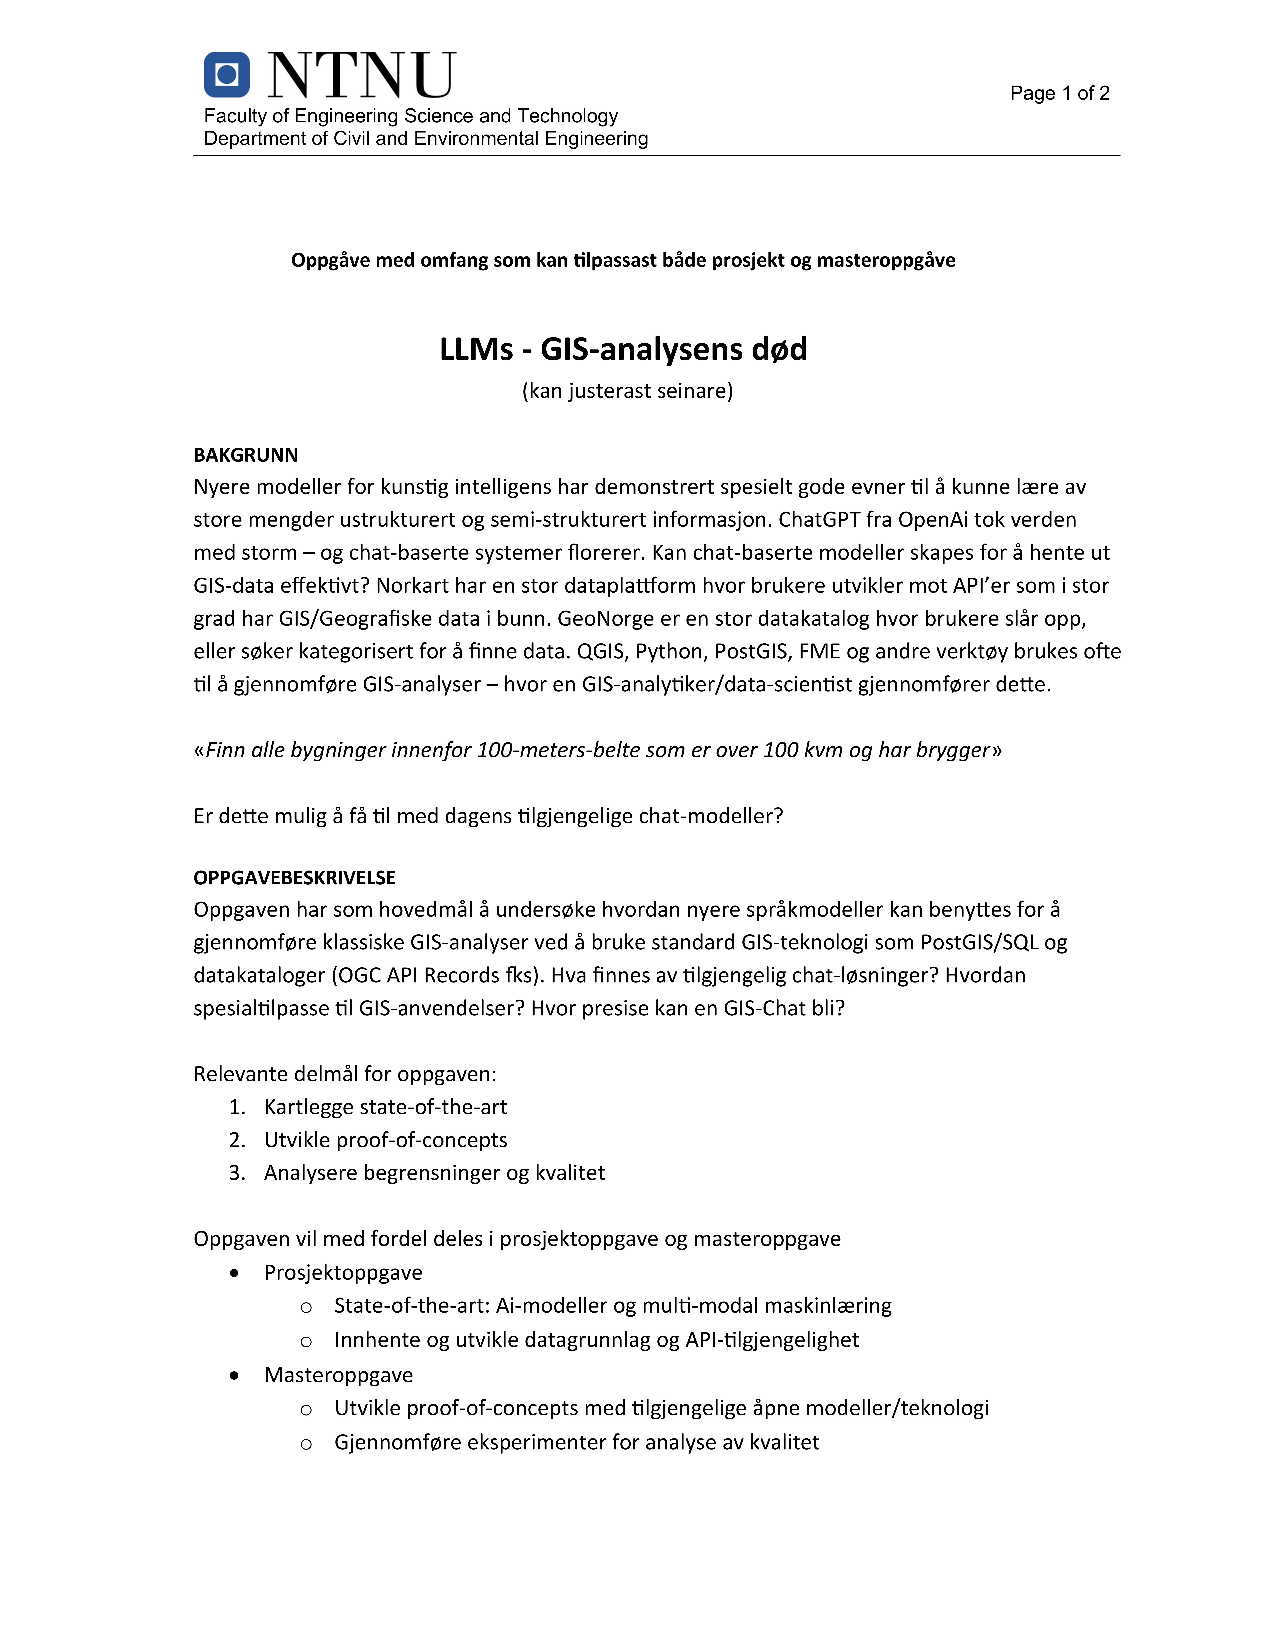
\includepdf[pages=1, scale=.7, pagecommand={\chapter{Task Description from Norkart}\label{app:task-description}}, linktodoc=true]{appendices/project_description.pdf}
    % \restoregeometry
    % \includepdf[pages=2-, scale=.7, pagecommand={}, linktodoc=true]{appendices/project_description.pdf}

    %     \chapter{API Schemas}

    %     \section[OGC API - Features]{\acrshort{acr:ogc} \acrshort{acr:api} - Features}

    %     \acrshort{acr:ogc} \acrshort{acr:api} specification for a 'collection' object\footnote{\url{https://schemas.opengis.net/ogcapi/features/part1/1.0/openapi/schemas/collection.yaml} (retrieved October 25, 2023)}:

    %     \begin{lstlisting}[style=yaml]
    %         type: object
    %         required:
    %         - id
    %         - links
    %         properties:
    %         id:
    %         description: identifier of the collection used, for example, in URIs
    %         type: string
    %         example: address
    %         title:
    %         description: human readable title of the collection
    %         type: string
    %         example: address
    %         description:
    %         description: a description of the features in the collection
    %         type: string
    %         example: An address.
    %         links:
    %         type: array
    %         items:
    %         $ref: link.yaml
    %     example:
    %       - href: http://data.example.com/buildings
    %       rel: item
    %       - href: http://example.com/concepts/buildings.html
    %       rel: describedby
    %         type: text/html
    %   extent:
    %     $ref: extent.yaml
    %   itemType:
    %   description: indicator about the type of the items in the collection (the default value is 'feature').
    %     type: string
    %     default: feature
    %     crs:
    %     description: the list of coordinate reference systems supported by the service
    %     type: array
    %     items:
    %       type: string
    %     default:
    %       - http://www.opengis.net/def/crs/OGC/1.3/CRS84
    %     example:
    %       - http://www.opengis.net/def/crs/OGC/1.3/CRS84
    %       - http://www.opengis.net/def/crs/EPSG/0/4326
    %     \end{lstlisting}

    %     \section[STAC API]{\acrshort{acr:stac} \acrshort{acr:api}}

    %     \chapter{Code Examples}

\end{appendix}

\clearpage
\printglossary[type=\acronymtype]

\end{document}
